%% For double-blind review submission, w/o CCS and ACM Reference (max submission space)
%\documentclass[sigplan,10pt,review,anonymous]{acmart}
%\settopmatter{printfolios=true,printccs=false,printacmref=false}
%% For double-blind review submission, w/ CCS and ACM Reference
%\documentclass[sigplan,review,anonymous]{acmart}\settopmatter{printfolios=true}
%% For single-blind review submission, w/o CCS and ACM Reference (max submission space)
%\documentclass[sigplan,review]{acmart}\settopmatter{printfolios=true,printccs=false,printacmref=false}
%% For single-blind review submission, w/ CCS and ACM Reference
%\documentclass[sigplan,review]{acmart}\settopmatter{printfolios=true}
%% For final camera-ready submission, w/ required CCS and ACM Reference
\documentclass[acmsmall]{acmart}\settopmatter{printccs=false,printacmref=false}


%% Conference information
%% Supplied to authors by publisher for camera-ready submission;
%% use defaults for review submission.
\acmConference{University of Michigan}{April, 2022}{Ann Arbor, MI, USA}
\acmISBN{} % \acmISBN{978-x-xxxx-xxxx-x/YY/MM}
\acmDOI{} % \acmDOI{10.1145/nnnnnnn.nnnnnnn}
\startPage{1}

%% Copyright information
%% Supplied to authors (based on authors' rights management selection;
%% see authors.acm.org) by publisher for camera-ready submission;
%% use 'none' for review submission.
\setcopyright{none}
%\setcopyright{acmcopyright}
%\setcopyright{acmlicensed}
%\setcopyright{rightsretained}
%\copyrightyear{2018}           %% If different from \acmYear

%% Bibliography style
\bibliographystyle{ACM-Reference-Format}
%% Citation style
\citestyle{acmauthoryear}  %% For author/year citations
%\citestyle{acmnumeric}     %% For numeric citations
%\setcitestyle{nosort}      %% With 'acmnumeric', to disable automatic
                            %% sorting of references within a single citation;
                            %% e.g., \cite{Smith99,Carpenter05,Baker12}
                            %% rendered as [14,5,2] rather than [2,5,14].
%\setcitesyle{nocompress}   %% With 'acmnumeric', to disable automatic
                            %% compression of sequential references within a
                            %% single citation;
                            %% e.g., \cite{Baker12,Baker14,Baker16}
                            %% rendered as [2,3,4] rather than [2-4].


%%%%%%%%%%%%%%%%%%%%%%%%%%%%%%%%%%%%%%%%%%%%%%%%%%%%%%%%%%%%%%%%%%%%%%
%% Note: Authors migrating a paper from traditional SIGPLAN
%% proceedings format to PACMPL format must update the
%% '\documentclass' and topmatter commands above; see
%% 'acmart-pacmpl-template.tex'.
%%%%%%%%%%%%%%%%%%%%%%%%%%%%%%%%%%%%%%%%%%%%%%%%%%%%%%%%%%%%%%%%%%%%%%


%% Some recommended packages.
\usepackage{booktabs}   %% For formal tables:
                        %% http://ctan.org/pkg/booktabs
\usepackage{subcaption} %% For complex figures with subfigures/subcaptions
                        %% http://ctan.org/pkg/subcaption
\usepackage[export]{adjustbox}

\usepackage[T1]{fontenc} % fix missing font cmtt
\usepackage{amsmath}
\let\Bbbk\relax
\usepackage{amssymb} % Vdash
\usepackage{graphicx} % rotatebox
\usepackage{stmaryrd} % llparenthesis
\usepackage{anyfontsize} % workaround for font size difference warning
\usepackage{todonotes}
\usepackage{listings}
\usepackage{tikz}
\usetikzlibrary{calc,fit,tikzmark,plotmarks,arrows.meta,positioning,overlay-beamer-styles}

\usepackage{cancel} % slash over symbol
\usepackage{hyperref}
\renewcommand\UrlFont{\color{blue}\rmfamily}
\def\figureautorefname{Fig.}
\def\lemmaautorefname{Lemma}
\def\sectionautorefname{Sec.}
\let\subsectionautorefname\sectionautorefname
\let\subsubsectionautorefname\sectionautorefname
\newcommand{\rulesref}[1]{Rules (\ref{#1})}
\newcommand{\ruleref}[1]{Rule (\ref{#1})}

\usepackage{xcolor}
\definecolor{hazelgreen}{RGB}{7,63,36}
\definecolor{hazellightgreen}{RGB}{103,138,97}
\definecolor{hazelyellow}{RGB}{245,222,179}
\definecolor{hazellightyellow}{RGB}{254,254,234}

\newcommand{\highlight}[1]{\colorbox{yellow}{$\displaystyle #1$}}

%% Jana Dunfield macros
\def\OPTIONConf{1}
\usepackage{jdunfield}
\usepackage{rulelinks}

\usepackage{listings}%
\lstloadlanguages{ML}
\lstset{tabsize=2, 
	basicstyle=\fontsize{7.5pt}{1em}\ttfamily, 
	% keywordstyle=\sffamily,
	commentstyle=\itshape\ttfamily\color{gray}, 
	stringstyle=\ttfamily\color{purple},
	mathescape=true,escapechar=\#,
	numbers=left, numberstyle=\scriptsize\color{gray}\ttfamily, language=ML, showspaces=false,showstringspaces=false,xleftmargin=15pt, 
	morekeywords={string, float, int, bool, match},
	classoffset=0,belowskip=\smallskipamount, aboveskip=\smallskipamount,
	moredelim=**[is][\color{red}]{SSTR}{ESTR}
}
\newcommand{\li}[1]{\lstinline[basicstyle=\ttfamily\fontsize{9pt}{1em}\selectfont]{#1}}
\newcommand{\lismall}[1]{\lstinline[basicstyle=\ttfamily\fontsize{9pt}{1em}\selectfont]{#1}}

% !TEX root = proposal.tex
\usepackage{centernot}
% reverse Vdash
\newcommand{\dashV}{\mathbin{\rotatebox[origin=c]{180}{$\Vdash$}}}

% Violet hotdogs; highlight color helps distinguish them
\newcommand{\llparenthesiscolor}{\textcolor{violet}{\llparenthesis}}
\newcommand{\rrparenthesiscolor}{\textcolor{violet}{\rrparenthesis}}

% HTyp and HExp
\newcommand{\hcomplete}[1]{#1~\mathsf{complete}}

% HTyp
\newcommand{\htau}{\dot{\tau}}
\newcommand{\tarr}[2]{\inparens{#1 \rightarrow #2}}
\newcommand{\tarrnp}[2]{#1 \rightarrow #2}
\newcommand{\trul}[2]{\inparens{#1 \Rightarrow #2}}
\newcommand{\trulnp}[2]{#1 \Rightarrow #2}
\newcommand{\tnum}{\mathtt{num}}
\newcommand{\tehole}{\llparenthesiscolor\rrparenthesiscolor}
\newcommand{\tsum}[2]{\inparens{#1 + #2}}
\newcommand{\tprod}[2]{\inparens{#1 \times #2}}
\newcommand{\tunit}{\mathtt{1}}
\newcommand{\tvoid}{\mathtt{0}}

\newcommand{\tlabeledsum}[1]{+\mathopen{}\left\{#1\right\}}

\newcommand{\tcompat}[2]{#1 \sim #2}
\newcommand{\tincompat}[2]{#1 \nsim #2}


% HTag
\newcommand{\tagC}{\underline{\mathbf{C}}}
\newcommand{\tagset}{\mathcal{C}}
\newcommand{\tagehole}[1]{\llparenthesiscolor\rrparenthesiscolor^{#1}}
\newcommand{\taghole}[2]{\llparenthesiscolor#1\rrparenthesiscolor^{#2}}

\newcommand{\tagmaymatch}[2]{#1 \mathbin{?} #2}

% HExp
\newcommand{\hexp}{\dot{e}}
\newcommand{\hlam}[3]{\lambda #1:#2.#3}
\newcommand{\hap}[2]{#1(#2)}
\newcommand{\hapP}[2]{(#1)~(#2)} % Extra paren around function term
\newcommand{\hnum}[1]{\underline{#1}}
\newcommand{\hadd}[2]{\inparens{#1 + #2}}
\newcommand{\hpair}[2]{(#1 , #2)}
\newcommand{\htriv}{()}
\newcommand{\hehole}[1]{\llparenthesiscolor\rrparenthesiscolor^{#1}}
\newcommand{\hhole}[2]{\llparenthesiscolor#1\rrparenthesiscolor^{#2}}
\newcommand{\heholep}[1]{\llparenthesiscolor\rrparenthesiscolor^{#1}}
\newcommand{\hholep}[3]{\llparenthesiscolor#1\rrparenthesiscolor^{#2}_{#3}}
\newcommand{\hindet}[1]{\lceil#1\rceil}
\newcommand{\hinj}[3]{\mathtt{inj}_{#1}^{#2}({#3})}
\newcommand{\hinl}[2]{\mathtt{inl}_{#1}({#2})}
\newcommand{\hinr}[2]{\mathtt{inr}_{#1}({#2})}
\newcommand{\hinjp}[2]{\mathtt{inj}_{#1}(#2)}
\newcommand{\hinlp}[1]{\mathtt{inl}(#1)}
\newcommand{\hinrp}[1]{\mathtt{inr}(#1)}
\newcommand{\hfst}[1]{\mathtt{fst}(#1)}
\newcommand{\hsnd}[1]{\mathtt{snd}(#1)}
\newcommand{\hmatch}[2]{\mathtt{match}(#1) \{#2\}}
\newcommand{\hcase}[5]{\mathtt{case}({#1},{#2}.{#3},{#4}.{#5})}
\newcommand{\hrules}[2]{#1 \mid #2}
\newcommand{\hrulesP}[2]{\inparens{#1 \mid #2}}
\newcommand{\hrul}[2]{#1 \Rightarrow #2}
\newcommand{\hrulP}[2]{\inparens{#1 \Rightarrow #2}}

\newcommand{\refutable}[1]{#1 ~\mathtt{refutable}_?}
\newcommand{\frefutable}[1]{\textit{refutable}_?\inparens{#1}}
\newcommand{\possible}[1]{#1 ~\mathtt{possible}}
\newcommand{\fpossible}[1]{\textit{possible}\inparens{#1}}
\newcommand{\inValues}[3]{#1 \in \mathtt{values}[#2]\inparens{#3}}

\newcommand{\hGamma}{\dot{\Gamma}}
\newcommand{\domof}[1]{\text{dom}(#1)}
\newcommand{\hsyn}[3]{#1 \vdash #2 \Rightarrow #3}
\newcommand{\hana}[3]{#1 \vdash #2 \Leftarrow #3}
\newcommand{\hexptyp}[4]{#1 \mathbin{;} #2 \vdash #3 : #4}
\newcommand{\hpattyp}[4]{#4 \vdash #1 : #2 \dashV #3}
\newcommand{\hsubstyp}[4]{#1 \mathbin{;} #2 \vdash #3 : #4}
\newcommand{\hpatmatch}[3]{#1 \vartriangleright #2 \dashV #3}
\newcommand{\hnotnotmatch}[2]{#1 \mathbin{\cancel{\bot}} #2}
\newcommand{\hnotmatch}[2]{#1 \mathbin{\bot} #2}
\newcommand{\hmaymatch}[2]{#1 \mathbin{?} #2}
\newcommand{\htrans}[2]{#1 \mapsto #2}
\newcommand{\hlongtrans}[2]{#1 \newline \mapsto #2}

\newcommand{\isVal}[1]{#1 ~\mathtt{val}}
\newcommand{\isErr}[1]{#1 ~\mathtt{err}}
\newcommand{\isIndet}[1]{#1 ~\mathtt{indet}}
\newcommand{\isFinal}[1]{#1 ~\mathtt{final}}
\newcommand{\notIntro}[1]{#1 ~\mathtt{notintro}}
\newcommand{\fnotIntro}[1]{\textit{notintro}\inparens{#1}}

\newcommand{\setof}[1]{\{#1\}}

% ZTyp and ZExp
\newcommand{\zlsel}[1]{{\bowtie}{#1}}
\newcommand{\zrsel}[1]{{#1}{\bowtie}}
\newcommand{\zwsel}[1]{
	\setlength{\fboxsep}{0pt}
	\colorbox{green!10!white!100}{
		\ensuremath{{{\textcolor{Green}{{\hspace{-2px}\triangleright}}}}{#1}{\textcolor{Green}{\triangleleft{\vphantom{\tehole}}}}}}
}

\newcommand{\removeSel}[1]{#1^{\diamond}}

% ZTyp
\newcommand{\ztau}{\hat{\tau}}

% ZExp
\newcommand{\zexp}{\hat{e}}

% rules with pointer

\newcommand{\zrulsP}[3]{\inparens{#1 \mid #2 \mid #3}}
\newcommand{\zruls}[3]{#1 \mid #2 \mid #3}
\newcommand{\zrules}{\hat{rs}}
\newcommand{\rmpointer}[1]{\inparens{#1}^\diamond}

% Constraint
\newcommand{\hxi}{\dot{\xi}}
\newcommand{\ctyp}[2]{#1 : #2}
\newcommand{\cdual}[1]{\overline{#1}}
\newcommand{\ctruify}[1]{\dot{\top}\inparens{#1}}
\newcommand{\cfalsify}[1]{\dot{\bot}\inparens{#1}}
\newcommand{\ctruth}{\top}
\newcommand{\cfalsity}{\bot}
\newcommand{\cnum}[1]{\underline{#1}}
\newcommand{\cnotnum}[1]{\underline{\cancel{#1}}}
\newcommand{\cunit}{()}
\newcommand{\cunknown}{\mathtt{?}}
\newcommand{\cor}[2]{#1 \vee #2}
\newcommand{\cand}[2]{#1 \wedge #2}
\newcommand{\cinj}[3]{\mathtt{inj}_{#1}^{#2}(#3)}
\newcommand{\notC}{\cancel{C}}
\newcommand{\nottagC}{\cancel{\tagC}}
\newcommand{\cinl}[1]{\mathtt{inl}(#1)}
\newcommand{\cinr}[1]{\mathtt{inr}(#1)}
\newcommand{\cpair}[2]{(#1 , #2)}
\newcommand{\csatisfy}[2]{#1 \models #2}
\newcommand{\cnotsatisfy}[2]{#1 \centernot{\models} #2}
\newcommand{\cmaysatisfy}[2]{#1 \models_{?} #2}
\newcommand{\cnotmaysatisfy}[2]{#1 \centernot{\models}_{?} #2}
\newcommand{\csatisfyormay}[2]{#1 \models_{?}^{\dag} #2}
\newcommand{\cnotsatisfyormay}[2]{#1 \centernot{\models}_{?}^{\dag} #2}
%temporary change, need to get it back to make appendix right
%\newcommand{\csatisfy}[2]{#1 \dot{\models} #2}
%\newcommand{\cnotsatisfy}[2]{#1 \centernot{\dot{\models}} #2}
%\newcommand{\cmaysatisfy}[2]{#1 \dot{\models}_{?} #2}
%\newcommand{\cnotmaysatisfy}[2]{#1 \centernot{\dot{\models}}_{?} #2}
%\newcommand{\csatisfyormay}[2]{#1 \dot{\models}_{?}^{\dag} #2}
%\newcommand{\cnotsatisfyormay}[2]{#1 \centernot{\dot{\models}}_{?}^{\dag} #2}
\newcommand{\ccsatisfy}[2]{#1 \models #2}
\newcommand{\ccnotsatisfy}[2]{#1 \centernot{\models} #2}
\newcommand{\cincon}[1]{#1 ~\mathtt{incon}}
\newcommand{\cmayincon}[1]{#1 ~\cancel{\mathtt{not~incon}}}

\newcommand{\fsatisfy}[2]{\textit{satisfy}\inparens{#1, #2}}
% !TeX root = thesis.tex
%% Statics

% typing of internal expressions
\newrulecommand{TVar}{TVar}
\newrulecommand{TNum}{TNum}
\newrulecommand{TLam}{TLam}
\newrulecommand{TAp}{TAp}
\newrulecommand{TPair}{TPair}
\newrulecommand{TFst}{TFst}
\newrulecommand{TSnd}{TSnd}
\newrulecommand{TInl}{TInl}
\newrulecommand{TInr}{TInr}
\newrulecommand{TMatchZPre}{TMatchZPre}
\newrulecommand{TMatchNZPre}{TMatchNZPre}
\newrulecommand{TEHole}{TEHole}
\newrulecommand{THole}{THole}

% typing of rule and rules
\newrulecommand{TRule}{TRule}
\newrulecommand{TOneRules}{TOneRules}
\newrulecommand{TRules}{TRules}

% typing of pattern
\newrulecommand{PTVar}{PTVar}
\newrulecommand{PTNum}{PTNum}
\newrulecommand{PTWild}{PTWild}
\newrulecommand{PTPair}{PTPair}
\newrulecommand{PTInl}{PTInl}
\newrulecommand{PTInr}{PTInr}
\newrulecommand{PTEHole}{PTEHole}
\newrulecommand{PTHole}{PTHole}

%% Dynamics

% typing of substitution
\newrulecommand{STEmpty}{STEmpty}
\newrulecommand{STExtend}{STExtend}

% syntactically not value
\newrulecommand{NVEHole}{NVEHole}
\newrulecommand{NVHole}{NVHole}
\newrulecommand{NVAp}{NVAp}
\newrulecommand{NVMatch}{NVMatch}
\newrulecommand{NVFst}{NVFst}
\newrulecommand{NVSnd}{NVSnd}

% refutable pattern
\newrulecommand{RNum}{RNum}
\newrulecommand{REHole}{REHole}
\newrulecommand{RHole}{RHole}
\newrulecommand{RInl}{RInl}
\newrulecommand{RInr}{RInr}
\newrulecommand{RPairL}{RPairL}
\newrulecommand{RPairR}{RPairR}

% refutable constraint
\newrulecommand{RXNum}{RXNum}
\newrulecommand{RXNotNum}{RXNotNum}
\newrulecommand{RXUnknown}{RXUnknown}
\newrulecommand{RXFalsity}{RXFalsity}
\newrulecommand{RXInl}{RXInl}
\newrulecommand{RXInr}{RXInr}
\newrulecommand{RXPairL}{RXPairL}
\newrulecommand{RXPairR}{RXPairR}

% possible constraint
\newrulecommand{PTruth}{PTruth}
\newrulecommand{PUnknown}{PUnknown}
\newrulecommand{PNum}{PNum}
\newrulecommand{PNotNum}{PNotNum}
\newrulecommand{PInl}{PInl}
\newrulecommand{PInr}{PInr}
\newrulecommand{PPair}{PPair}
\newrulecommand{POrL}{POrL}
\newrulecommand{POrR}{POrR}

% match
\newrulecommand{MVar}{MVar}
\newrulecommand{MNum}{MNum}
\newrulecommand{MWild}{MWild}
\newrulecommand{MPair}{MPair}
\newrulecommand{MNotIntroPair}{MNotIntroPair}
\newrulecommand{MInl}{MInl}
\newrulecommand{MInr}{MInr}

% may match
\newrulecommand{MMEHole}{MMEHole}
\newrulecommand{MMHole}{MMHole}
\newrulecommand{MMNotIntro}{MMNotIntro}
\newrulecommand{MMPairL}{MMPairL}
\newrulecommand{MMPairR}{MMPairR}
\newrulecommand{MMPair}{MMPair}
\newrulecommand{MMInl}{MMInl}
\newrulecommand{MMInr}{MMInr}

% not match
\newrulecommand{NMNum}{NMNum}
\newrulecommand{NMPairL}{NMPairL}
\newrulecommand{NMPairR}{NMPairR}
\newrulecommand{NMConfL}{NMConfL}
\newrulecommand{NMConfR}{NMConfR}
\newrulecommand{NMInl}{NMInl}
\newrulecommand{NMInr}{NMInr}

% value
\newrulecommand{VNum}{VNum}
\newrulecommand{VLam}{VLam}
\newrulecommand{VPair}{VPair}
\newrulecommand{VInl}{VInl}
\newrulecommand{VInr}{VInr}

% indeterminate
\newrulecommand{IEHole}{IEHole}
\newrulecommand{IHole}{IHole}
\newrulecommand{IAp}{IAp}
\newrulecommand{IPairL}{IPairL}
\newrulecommand{IPairR}{IPairR}
\newrulecommand{IPair}{IPair}
\newrulecommand{IFst}{IFst}
\newrulecommand{ISnd}{ISnd}
\newrulecommand{IInl}{IInl}
\newrulecommand{IInr}{IInr}
\newrulecommand{IMatch}{IMatch}

% final
\newrulecommand{FVal}{FVal}
\newrulecommand{FIndet}{FIndet}

% step
\newrulecommand{ITHole}{ITHole}
\newrulecommand{ITApFun}{ITApFun}
\newrulecommand{ITApArg}{ITApArg}
\newrulecommand{ITAp}{ITAp}
\newrulecommand{ITPairL}{ITPairL}
\newrulecommand{ITPairR}{ITPairR}
\newrulecommand{ITFst}{ITFst}
\newrulecommand{ITSnd}{ITSnd}
\newrulecommand{ITFstPair}{ITFstPair}
\newrulecommand{ITSndPair}{ITSndPair}
\newrulecommand{ITInl}{ITInl}
\newrulecommand{ITInr}{ITInr}
\newrulecommand{ITExpMatch}{ITExpMatch}
\newrulecommand{ITSuccMatch}{ITSuccMatch}
\newrulecommand{ITFailMatch}{ITFailMatch}

% typing of constraints
\newrulecommand{CTTruth}{CTTruth}
\newrulecommand{CTFalsity}{CTFalsity}
\newrulecommand{CTUnknown}{CTUnknown}
\newrulecommand{CTNum}{CTNum}
\newrulecommand{CTNotNum}{CTNotNum}
\newrulecommand{CTAnd}{CTAnd}
\newrulecommand{CTOr}{CTOr}
\newrulecommand{CTInl}{CTInl}
\newrulecommand{CTInr}{CTInr}
\newrulecommand{CTPair}{CTPair}

% satisfaction judgment
\newrulecommand{CSTruth}{CSTruth}
\newrulecommand{CSNum}{CSNum}
\newrulecommand{CSNotNum}{CSNotNum}
\newrulecommand{CSAnd}{CSAnd}
\newrulecommandONE{CSOrL}{CSOrL}
\newrulecommandONE{CSOrR}{CSOrR}
\newrulecommand{CSInl}{CSInl}
\newrulecommand{CSInr}{CSInr}
\newrulecommand{CSPair}{CSPair}
\newrulecommand{CSNotIntroPair}{CSNotIntroPair}

% maybe satisfaction judgment
\newrulecommand{CMSUnknown}{CMSUnknown}
\newrulecommand{CMSNotIntro}{CMSNotIntro}
\newrulecommand{CMSAndL}{CMSAndL}
\newrulecommand{CMSAndR}{CMSAndR}
\newrulecommand{CMSAnd}{CMSAnd}
\newrulecommand{CMSOrL}{CMSOrL}
\newrulecommand{CMSOrR}{CMSOrR}
\newrulecommand{CMSInl}{CMSInl}
\newrulecommand{CMSInr}{CMSInr}
\newrulecommand{CMSPairL}{CMSPairL}
\newrulecommand{CMSPairR}{CMSPairR}
\newrulecommand{CMSPair}{CMSPair}

% must or maybe satisfaction judgment
\newrulecommand{CSMSMay}{CSMSMay}
\newrulecommand{CSMSSat}{CSMSSat}

% incon
\newrulecommand{CINCTruth}{CINCTruth}
\newrulecommand{CINCFalsity}{CINCFalsity}
\newrulecommand{CINCNum}{CINCNum}
\newrulecommand{CINCNotNum}{CINCNotNum}
\newrulecommand{CINCAnd}{CINCAnd}
\newrulecommand{CINCOr}{CINCOr}
\newrulecommand{CINCInj}{CINCInj}
\newrulecommand{CINCInl}{CINCInl}
\newrulecommand{CINCInr}{CINCInr}
\newrulecommand{CINCPairL}{CINCPairL}
\newrulecommand{CINCPairR}{CINCPairR}

%% labeled sum dynamics
\newrulecommand{ITInj}{ITInj}
\newrulecommand{VInj}{VInj}
\newrulecommand{IEInj}{IEInj}
\newrulecommand{IEInjHole}{IEInjHole}
\newrulecommand{MInj}{MInj}
\newrulecommand{NMInj}{NMInj}
\newrulecommand{NMInjTag}{NMInjTag}
\newrulecommand{NMInjArg}{NMInjArg}
\newrulecommand{MMInjTag}{MMInjTag}
\newrulecommand{MMInjArg}{MMInjArg}
\newrulecommand{TMMSym}{TMMSym}
\newrulecommand{TMMHole}{TMMHole}
\newrulecommand{TMMEHole}{TMMEHole}
\newrulecommand{TNMTag}{TNMTag}
\newrulecommand{RInjSing}{RInjSing}
\newrulecommand{RInjMult}{RInjMult}

% labeled sum statics
\newrulecommand{TInj}{TInj}
\newrulecommand{PTInj}{PTInj}
\newrulecommand{CTInj}{CTInj}
\newrulecommand{RXInj}{RXInj}
\newrulecommand{PInj}{PInj}
\newrulecommand{CSInj}{CSInj}
\newrulecommand{CMSInjTag}{CMSInjTag}
\newrulecommand{CMSInjArg}{CMSInjArg}

% labeled sum incon
\newrulecommand{CINCInjTag}{CINCInjTag}
\newrulecommand{CINCInjArg}{CINCInjArg}

% Curry-Howard Correspondence
\newrulecommand{AndIntro}{AndIntro}
\newrulecommand{AndElimL}{AndElimL}
\newrulecommand{AndElimR}{AndElimR}
\newrulecommand{TAPair}{TAPair}
\newrulecommand{TAFst}{TAFst}
\newrulecommand{TASnd}{TASnd}

\newrulecommand{UniversalIntro}{UniversalIntro}
\newrulecommand{UniversalElim}{UniversalElim}
\newrulecommand{TALam}{TALam}
\newrulecommand{TAAp}{TAAp}

% Agda examples
\newrulecommand{Zero}{Zero}
\newrulecommand{Suc}{Suc}
\newrulecommand{ZLessThanS}{Z<S}
\newrulecommand{SLessThanS}{S<S}

% BadRules
\newrulecommand{BadTRule}{BadTRule}
\newrulecommand{GoodTRule}{GoodTRule}


\begin{document}

%% Title information
\title{Pattern Matching with Typed Holes}         %% [Short Title] is optional;
                                        %% when present, will be used in
                                        %% header instead of Full Title.
                                        %% contents suppressed with 'anonymous'
\subtitle{Computer Science Honors Thesis}                     %% \subtitle is optional
                                        %% can be repeated if necessary;
                                        %% contents suppressed with 'anonymous'


%% Author information
%% Contents and number of authors suppressed with 'anonymous'.
%% Each author should be introduced by \author, followed by
%% \authornote (optional), \orcid (optional), \affiliation, and
%% \email.
%% An author may have multiple affiliations and/or emails; repeat the
%% appropriate command.
%% Many elements are not rendered, but should be provided for metadata
%% extraction tools.

%% Author with single affiliation.
\author{Scott Guest}
\orcid{nnnn-nnnn-nnnn-nnnn}             %% \orcid is optional
\affiliation{
  \institution{University of Michigan}            %% \institution is required
}
\email{sguest@umich.edu}          %% \email is recommended

%% Author with two affiliations and emails.
\author{Cyrus Omar}
\affiliation{
  \institution{University of Michigan}           %% \institution is required
}
\email{comar@umich.edu}         %% \email is recommended


%% Abstract
%% Note: \begin{abstract}...\end{abstract} environment must come
%% before \maketitle command
\begin{abstract}
	To support reasoning about incomplete programs in a principled way, various programming systems have introduced \emph{typed-holes} - placeholder terms which indicate missing syntactic pieces or semantic inconsistencies \cite{GHCHoles, DBLP:journals/jfp/Brady13, DBLP:conf/icfp/Norell13, DBLP:conf/popl/OmarVHAH17}. Ideally, these holes allow every intermediate edit state of a program to be given static or even dynamic meaning, with the aim of enabling simpler and more powerful development tools \cite{DBLP:conf/snapl/OmarVHSGAH17, DBLP:journals/pacmpl/OmarVCH19}. However, current systems are limited in that they only support holes in expressions or types, presenting difficulty when editing binding constructs such as patterns. To resolve this, we have developed Peanut: a calculus for pattern matching with typed pattern holes, including support for exhaustiveness and redundancy checking in this setting. Additionally, we also provide a mechanization of Peanut's semantics and metatheory in the Agda proof-assistant \cite{norell:thesis}.
\end{abstract}
%% End of generated code


%% \maketitle
%% Note: \maketitle command must come after title commands, author
%% commands, abstract environment, Computing Classification System
%% environment and commands, and keywords command.
\maketitle

\section{Introduction}\label{sec:intro}

For the modern programmer, development has progressed beyond the unassisted writing of code in a text editor, and it now increasingly involves conversing with a wide-variety of programming tools. As incremental changes are made, type checkers, debuggers, interpreters, program synthesizers and so forth all provide feedback, seeking to increase programmer productivity or ensure program correctness. Unfortunately, however, programming languages typically only assign meaning to programs which are already fully-formed and well-typed. As a result, these tools struggle to deal with what is perhaps one of the most common states of a program during development: an unfinished piece of work with ongoing, syntax-breaking editing or as-yet-unresolved semantic errors. Throughout the editing process then, feedback from these tools is only available sporadically, limiting their usefulness when they are needed most.

This troublesome issue, where programming tools have gaps in their services throughout the editing process, is aptly known as the \emph{gap problem}. Previously, most attempts to close such gaps have relied on \textit{ad hoc} or fragile heuristics, for example, making assumptions about missing tokens, or ignoring large swathes of invalid code all together \cite{DBLP:conf/oopsla/KatsJNV09, DBLP:conf/snapl/OmarVHSGAH17}. Recently though, the work of  \cite{DBLP:conf/snapl/OmarVHSGAH17} has outlined a more principled approach: rather than treating intermediate edit states as meaningless, one can extend a language's syntax and semantics to explicitly represent all such states as well-formed terms. Every editor state can then be assigned static or even dynamic meaning, allowing programming tools to handle them in a uniform way and removing the need for such \emph{ad hoc} heuristics.

To varying degree, systems including Haskell \cite{GHCHoles}, Idris \cite{DBLP:journals/jfp/Brady13}, Agda \cite{DBLP:conf/icfp/Norell13}, and Hazel \cite{DBLP:conf/popl/OmarVHAH17} implement this approach through a feature known as \emph{typed-holes}. When a program has a missing syntactic piece, rather than treating the entire program as meaningless, we localize the issue by inserting an \emph{empty hole} expression at the unfinished location. Likewise, semantically inconsistent expressions, e.g. those that are ill-typed or reference undefined identifiers, may be wrapped with a \emph{non-empty hole} expression, isolating the inconsistency from the program at large. Tools can then the aid the developer by providing static information about these holes - displaying the variables and types in scope, inferring the expected type, or even synthesizing possible hole-fillings \cite{DBLP:conf/haskell/Gissurarson18, DBLP:journals/pacmpl/LubinCOC20}. 

\begin{figure}
	\centering
	\subcaptionbox{Empty and non-empty holes\label{fig:arith-initial}}{
		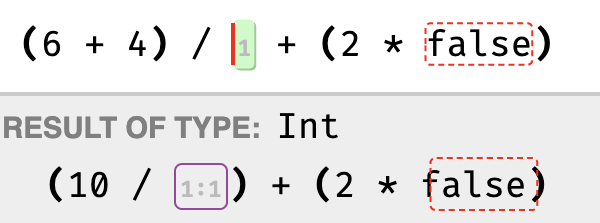
\includegraphics[scale=0.47,valign=t]{imgs/arith-initial.png}%
		\vphantom{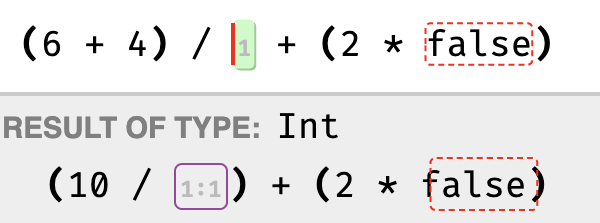
\includegraphics[scale=0.47,valign=t]{imgs/arith-initial.png}}
	}
	\hfil
	\subcaptionbox{Result after filling empty hole\label{fig:arith-partial}}{
		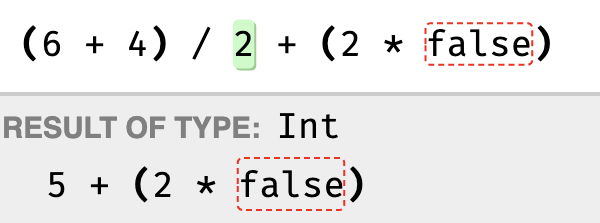
\includegraphics[scale=0.47,valign=t]{imgs/arith-partial.png}%
	 	\vphantom{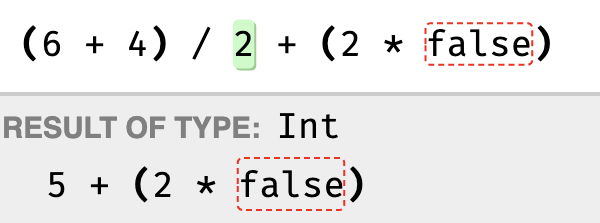
\includegraphics[scale=0.47,valign=t]{imgs/arith-partial.png}}
	}
	\hfil\par\bigskip
	\subcaptionbox{Result after filling non-empty hole\label{fig:arith-complete}}{
		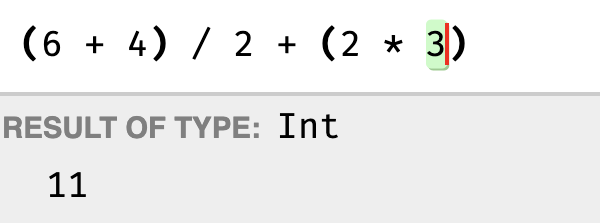
\includegraphics[scale=0.47,valign=t]{imgs/arith-complete.png}
	}
	\caption{Live Evaluation with Expression Holes}
	\label{fig:arith-example}
\end{figure}

Most notable among the aforementioned systems is Hazel - a structure editor which was designed from logical and type-theoretic first principles to seamlessly and fully-automatically insert holes throughout the editing process. Starting from an empty hole, every possible program can be built up using a set of edit actions which directly manipulate the syntax tree. Along the way, Hazel maintains a \emph{maximal liveness} invariant so that every intermediate step is a valid term with well-defined static and dynamic semantics, completely eliminating the gap problem \cite{DBLP:journals/pacmpl/OmarVCH19}. \autoref{fig:arith-example} displays screenshots of a small part of the Hazel editor, with the user in the process of editing a simple arithmetic expression. Considering only Fig.~\ref{fig:arith-initial} for now, both variants of typed-holes are present: an empty hole labeled with id \li{1} indicates a missing piece of the expression, and a non-empty hole, shown as a dashed red box, serves as a membrane around the type inconsistency related to the term \li{false}.

One of  Hazel's main contributions is its comprehensive dynamic semantics which allows evaluation to continue "around holes", thereby preventing gaps in services which rely on actual program execution \cite{DBLP:journals/pacmpl/OmarVCH19}. This stands in contrast to systems such as Haskell, which, when supplied with appropriate compiler flags, treat holes as panics - reminiscent of a common pattern where developers raise an exception at yet-to-be-implemented code locations \cite{GHCHoles}. With Hazel, however, upon evaluation encountering a hole, rather than panicking or otherwise terminating the program, Hazel defers the evaluation of that particular expression and those that rely on. It then continues to evaluate all other complete (i.e. hole-less) parts of the program until no such evaluation is possible. Finally, evaluation pauses, yielding an \emph{indeterminate} value if there are still holes present. At a later time, the remaining holes in this indeterminate result can be filled, and evaluation resumes without having to restart the program. As a result, Hazel provides continuous live feedback throughout the entire editing process.

The rest of \autoref{fig:arith-example} demonstrates this live evaluation. Initially, the expression shown in Fig.~\ref{fig:arith-initial} contains two holes. Hazel partially evaluates the expression, reducing the complete term \li{6 + 4} to \li{10}, but can perform no further reductions. An indeterminate result is displayed, still containing both holes present in the initial expression. In Fig.~\ref{fig:arith-partial}, we then fill the empty hole with id \li{1} using the value \li{2}. This allows evaluation to resume, further reducing \li{(6 + 4) / 2} to \li{5}, but again pausing due to the presence of the non-empty hole. Finally, in Fig.~\ref{fig:arith-complete}, we resolve the typing inconsistency by replacing the term \li{false} with the integer \li{3}. The non-empty hole is automatically removed, and Hazel now produces a concrete value \li{11}. At no point during this process is the editor state meaningless, nor is the program ever restarted.

While Hazel itself is still under development, and is currently little more than a lambda calculus with primitive types, sums, and products, it seeks to soon reach feature-parity with production-level languages such as Elm \cite{DBLP:conf/pldi/CzaplickiC13, Elm, DBLP:journals/pacmpl/OmarVCH19}. Indeed, the machinery behind Hazel is not limited to its specific features, but rather, it provides a systematic, near-mechanical way to build similar structure editors for any language. Its semantics are built up using common techniques from gradual typing \cite{DBLP:conf/snapl/SiekVCB15}: holes are considered to have the unknown type, and terms are elaborated into a cast calculus to handle such typing at runtime. Additional machinery from contextual modal type theory \cite{DBLP:journals/tocl/NanevskiPP08} is then used to track substitutions which occur around holes, allowing holes to be filled in any order while producing the same final result. Given this principled theoretical basis, future work may even allow us to algorithmically generate Hazel-like structure editors for numerous languages in a fully automatic way, developing something akin to the Gradualizer \cite{DBLP:conf/popl/CiminiS16}. However, for any of this development be possible, and indeed to apply Hazel's techniques to any full-fledged functional programming language at all, one commonplace feature still needs more careful consideration: \emph{structural pattern matching}.

Throughout the rest of this paper, we tackle the challenge of integrating pattern matching into a Hazel-like system while seeking to maintain the maximal liveness invariant. We begin in \autoref{sec:background} by reviewing the required background and terminology for pattern matching in general. In \autoref{sec:pattern-matching}, we then introduce the concept of a \emph{pattern hole}, and provide a high-level discussion of our desired semantics for pattern matching with these holes, including redundancy and exhaustiveness in this setting. Finally,  in \autoref{sec:peanut}, we formalize this high-level discussion, presenting our work as a type theoretic calculus Peanut which extends the Hazelnut Live internal language 
of \cite{DBLP:journals/pacmpl/OmarVCH19}. To round off the development, we also outline algorithmic implementations of redundancy and exhaustiveness checking in \autoref{sec:decidability}, then discuss an Agda mechanization of Peanut's semantics and metatheory in \autoref{sec:mechanization}.

\section{Background}\label{sec:background}

Let us begin by reviewing pattern matching in the context of languages without holes. Such a feature should be familiar to many modern developers, as it has seen widespread adoption in typed functional languages such as OCaml \cite{leroy:hal-00930213}, Haskell \cite{marlow2010haskell}, and Elm \cite{Elm}, and more recently, has also been implemented to varying degree in mainstream imperative languages including Rust \cite{10.5555/3271463} and Python \cite{pep634}, and has also been proposed for a future version of C++ \cite{murzin2019pattern}.

At a high-level, \emph{structural pattern matching} allows one to conditionally branch based on the "shape" of a piece of data, while simultaneously binding sub-terms of the data to specified variable names. Concretely, this accomplished through a \li{match} expression consisting of a \emph{scrutinee}, i.e. the expression whose shape we inspect, and a series of \emph{rules}. Each rule contains a \emph{pattern} describing the desired form of the data for that particular case, as well as a \emph{branch expression} indicating the result of evaluation in that case. The branch expression may reference the variables bound  in the pattern.

\begin{figure}
	\begin{subfigure}{.45\textwidth}
		\begin{lstlisting}[numbers=none]
			match tree
			| Node([]) -> Empty
			| Node([x]) -> Node([f x, Empty])
			| Node([x, y]) -> Node([f x, f y])
			| Node(x::y::tl) -> Node(
			[f x, f (Node (y::tl))])
			| Leaf x -> Leaf x
			| Empty -> Empty
			end
		\end{lstlisting}
		\caption{Exhaustive + Irredundant\label{fig:basic-examples-correct}}
	\end{subfigure}
	\begin{subfigure}{.5\textwidth}
		\begin{lstlisting}[numbers=none]
			match tree
			| Node(x::y::tl) -> Node(
			[f x, f (Node (y::tl))])
			| Node([x, y]) -> Node([f x, f y])
			| Node([x]) -> Node([f x, Empty])
			| Node([]) -> Empty
			| Empty -> Empty
			end
			##
		\end{lstlisting}
		\caption{Inexhaustive + Redundant (Second Pattern)\label{fig:basic-examples-wrong}}
	\end{subfigure}
	\caption{Two examples demonstrating structural pattern matching and common pitfalls.}
	\label{fig:basic-examples}
\end{figure}

\autoref{fig:basic-examples-correct} and \autoref{fig:basic-examples-wrong} present pseudocode showcasing this feature. The scrutinee is a variable \li{tree} containing some value of an algebraic datatype. Each pattern is an expression of nested constructors that could possibly match those constructors of the value in \li{tree}, with variable names in a pattern acting similarly to a wildcard. Semantically, the match expression compares the value of \li{tree} against each of these patterns, beginning from the top down. The first pattern accurately describing the constructors in \li{tree} is selected, then variables in the pattern are bound to corresponding sub-terms of \li{tree}, and finally, evaluation continues at the selected branch expression. 

Explicitly, in \autoref{fig:basic-examples-correct}, assume \li{tree} contains the value \li{Node([Foo(4), Bar(5)])}, where the syntax \li{[x , y]} is sugar for the nested cons cells \li{x::y::[]}. Although the first two patterns indeed have an outermost \li{Node} constructor, they are not matched due to the inner list constructors differing from our value. However, the third pattern \li{Node([x, y])} is successfully matched, thereby binding the variable \li{x} to \li{Foo(4)} and the variable \li{y} to \li{Bar(5)}. Correspondingly, the whole term evaluates to the branch expression \li{Node([f(Foo(4)), f(Bar(5))])}. Note that our scrutinee would also match the fourth pattern \li{Node(x::y::tl)} - binding \li{x} to \li{Foo(4)}, \li{y} to \li{Bar(5)}, and \li{tl} to \li{[]}. However, execution does not actually reach this point, as the third pattern is matched earlier in the rule sequence.

More than just a useful control flow structure, pattern matching also helps to ensure program correctness. Consider if  the user modifies \autoref{fig:basic-examples-correct} to the program shown in \autoref{fig:basic-examples-wrong}. For our previously discussed value, the new ordering of rules results in the pattern \li{Node(x::y::tl)} being matched before the pattern \li{Node([x, y])} is ever considered, changing the overall behavior of the program. In fact, any scrutinee which matches the second pattern \li{Node([x, y])} will also match the first pattern \li{Node(x::y::tl)}. Resultingly, as evaluation considers rules top to bottom, the second pattern here is unreachable and entirely \emph{redundant}. Such a bug caused by reordering can be quite subtle, and it would be difficult to detect if our program had instead been formulated using, say, a series of \li{if}-\li{then}-\li{else} expressions. However, with pattern matching, we can easily prevent such issues by performing \emph{redundancy analysis} -  an algorithm which allows the language to statically detect if any rule in a \li{match} is impossible to reach due to it being entirely subsumed by earlier rules in the sequence. The user can then be notified of a likely bug, eliminating large classes of errors related to code reordering or unused code paths.

Additionally, note that \autoref{fig:basic-examples-wrong} also fails to include the \li{Leaf x} pattern, meaning that certain scrutinee values will no longer match any of the given cases. By performing \emph{exhaustiveness analysis}, we can prevent this issue as well, statically checking that every expression of a given type matches at least one of the patterns in a \li{match} expression. As a result, the programmer is forced to handle every possible form of an input, and if they fail to do so, the language can often assist them by generating expressions which are not yet handled \cite{Harper2012}. Again, this enables large classes of bugs to be prevented statically. For example, from a certain viewpoint, common security issues such as null-pointer exceptions can be viewed as a failure to check exhaustiveness. Exhaustiveness also aids refactoring: if a datatype is extended with additional constructors, then the language can statically identify every location where these additional constructors must be handled. 

Anecdotally, the author's found these analyses immensely useful during the development of the Agda mechanization discussed in \autoref{sec:mechanization}. In the context of Agda and other dependently typed theorem provers, exhaustiveness is used to ensure totality, in effect, guaranteeing that every proof handles all necessary cases. When, for example, we added a unit type to our development after an initial mechanization had already been completed, this removed the need to manually track down and identify all proofs that needed to be updated. Instead, all that was necessary was to one-by-one handle every inexhaustiveness error reported by the compiler.
\section{Pattern Matching with Typed Holes in Hazel}\label{sec:pattern-matching}

Let us now return to the problem of extending Hazel with pattern matching, placing particular emphasis on maintaining Hazel's maximal liveness invariant. Presently, all current systems with typed-holes only support holes in expressions or types, but notably, do not permit holes in binding constructs such as patterns. As a result, when editing a pattern - a necessarily incremental process - a user still faces meaningless editor states and thus gaps in editor services. To resolve this, we again turn to the approach outlined in \cite{DBLP:conf/snapl/OmarVHSGAH17}, extending our language to represent such intermediate pattern edit states as well-formed terms. 

Note that, for our purposes, patterns and expressions are quite similar: both are built up compositionally and are subject to typing restrictions. Correspondingly, we proceed by introducing two variants of \emph{pattern holes}. We include \emph{empty pattern holes} to indicate a missing sub-term of a pattern, and we include \emph{non-empty pattern holes} to act as a membrane around patterns that are ill-typed with regards to their location in a larger pattern. Syntactically, pattern holes indeed enable us to represent any pattern edit state without much difficulty, and they are fairly trivial to implement into our extension of Hazel. Semantically, however, the situation is much more subtle. 

At a high level, expression holes indicate \emph{unknown expressions} and pattern holes indicate \emph{unknown patterns}. Thus, whatever semantics we choose to give terms with holes, it must be sound with respect to all possible hole fillings, and resultingly, we must reason conservatively about the contents of any particular hole. At the same time, we must strike a balance, limiting this conservativeness as much as possible in order to still provide viable static analysis and dynamic evaluation in cases where we can soundly do so without knowledge about the contents of any hole. For pattern matching, this balance manifests as stating that a match succeeds only if it succeeds in all possible (expression and pattern) hole fillings. Likewise, a match fails only if it fails in all possible hole fillings. However, as the astute reader will note, this leaves open a third possibility: some hole fillings may result in a match succeeding while other hole fillings result in the match failing - an expression may \emph{indeterminately} match a pattern. 

When we allow expression and pattern holes, we can then no longer determinately say whether an expression matches a given pattern. What was once a binary decision - either $e$ matches $p$ or $e$ does not match $p$ - is now a ternary decision: either $e$ must match $p$, $e$ must not match $p$, or $e$ indeterminately matches $p$ depending on how the various holes are filled. In turn, redundancy and exhaustiveness also become ternary decisions: a \li{match} expression may either be necessarily exhaustive, necessarily inexhaustive, or indeterminate, and likewise for redundancy. To more concretely present these subtleties, we now discuss the running example of an \li{odd_length} function which returns whether an input of type \li{[Int]} has an odd number of elements. We explore the full semantics of the \li{match} expression with live evaluation in \autoref{sec:live-eval}, then further explore exhaustiveness in \autoref{sec:exhaustiveness} and redundancy in \autoref{sec:redundancy}.

\subsection{Live Evaluation with Pattern Holes}\label{sec:live-eval}

As discussed, in order to support live evaluation with pattern holes, we must distinguish whether a given expression and pattern \emph{must} match, \emph{must not} match, or \emph{indeterminately} match. Let us consider how these different possibilities play out in \autoref{fig:evaluation-ex}, working through examples of a \li{match} expression with expression holes in the scrutinee and with pattern holes in the listed rules. The provided screenshots are from our Hazel implementation of this feature.

\begin{figure}
	\centering
	% Capture tallest image in box 2
	\setbox2=\hbox{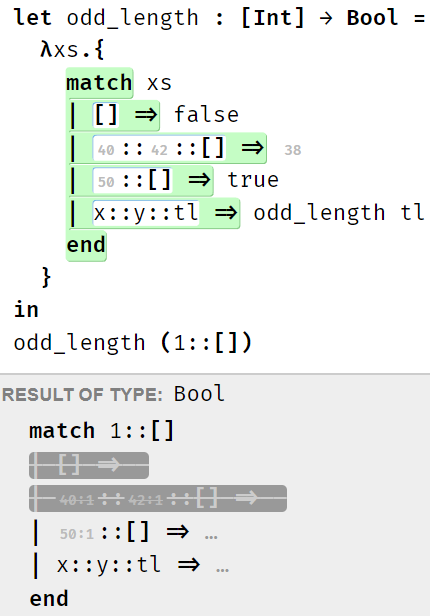
\includegraphics[scale=0.47]{imgs/pat_match_pat_holes.png}}%
	\subcaptionbox{Pattern matching with expression holes\label{fig:exp-hole}}{
		\raisebox{\dimexpr\ht2-\height}{
			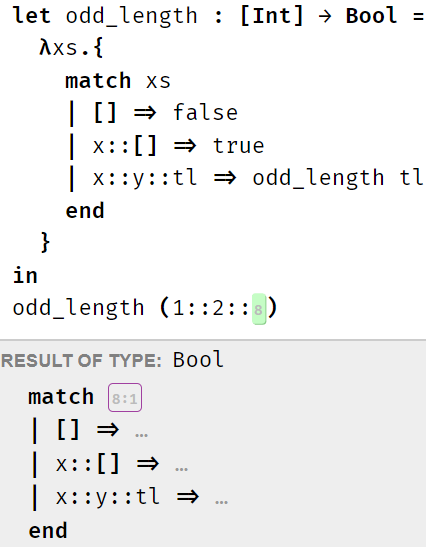
\includegraphics[scale=0.47,valign=t]{imgs/pat_match_exp_holes.png}
			\vphantom{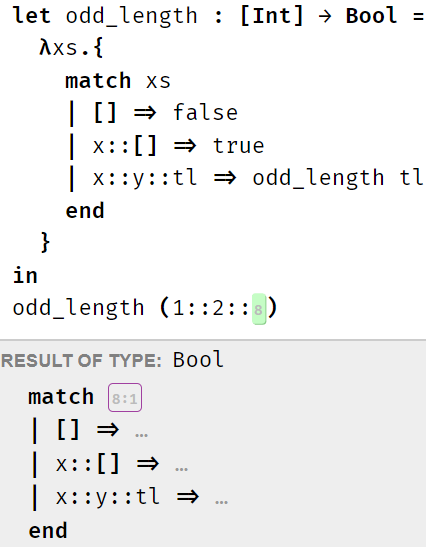
\includegraphics[scale=0.47,valign=t]{imgs/pat_match_exp_holes.png}}
		}
	}
	\hfil
	\subcaptionbox{Pattern matching with pattern holes\label{fig:pat-hole}}{
		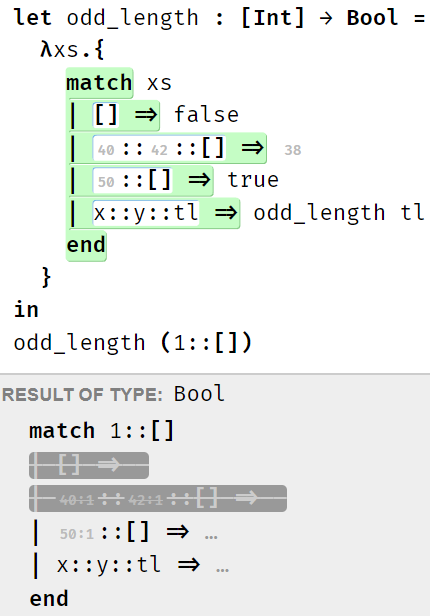
\includegraphics[scale=0.47,valign=t]{imgs/pat_match_pat_holes.png}
	}
	\caption{Live Evaluation with Expression and Pattern Holes}
	\label{fig:evaluation-ex}
\end{figure}


In \autoref{fig:exp-hole}, we apply the function \li{odd_length} to an argument that contains an expression hole with id \li{8}. Although the argument is indeterminate and cannot be fully-evaluated, per Hazel's live dynamic semantics, we substitute the partially evaluated argument into the function body and continue as far as possible. The argument then becomes the scrutinee of our \li{match} expression, and we proceed with pattern matching. Beginning with the first pattern, regardless of hole filling, the outermost constructor of our scrutinee is always a cons operator \li{::} rather than the empty list \li{[]}. Thus, our scrutinee must not match the first pattern \li{[]}, and we continue to the next rule. For the second pattern, our scrutinee always contains at least two elements while the pattern specifies only one element, so again, the expression must not match, and evaluation move to consider the third pattern. In this case, as the scrutineee indeed always contains at least two elements, the third match finally succeeds. Correspondingly, \li{x} is bound to \li{1}, \li{y} is bound to \li{2}, and \li{tl} is bound to the hole with id \li{8}. Evaluation then proceeds to the recursive call, and in this frame, our scrutinee becomes just an expression hole. Because we do not know whether the hole will be filled with an empty list or some other contents, we cannot determinately say whether it matches the pattern \li{[]}, hence evaluation must pause. We cannot proceed without further hole filling, so the entire \li{match} expression becomes indeterminate, displayed as the final result at the bottom of the image. Note that the scrutinee in the final result is indeed just the expression hole with id \li{8}.

In \autoref{fig:pat-hole}, our argument no longer contains any expression holes, but indeterminacy still arises due to the pattern holes in the second and third rules of the \li{match} expression. Specifically, evaluation begins by analyzing the scrutinee against the first pattern, and as \li{1 :: []} is not the empty list, we determine it must not match the first pattern. Likewise, despite the presence of pattern holes, the second pattern may only be matched by a two element list, so our scrutinee must not match it, and we continue to the third pattern. The third pattern gives the most interesting case. It indeed specifies a list with a single element, but the head of the pattern is a  pattern hole with id \li{50}, indicating that the first element of the scrutinee must match some yet-unknown pattern. If hole \li{50} were filled with the integer pattern \li{1} or a variable \li{x}, then \li{1::[]} would match. However, for many other hole fillings, e.g. the integer \li{2}, the match clearly fails. As a result, we can only state that \li{1::[]} indeterminately matches the third pattern, and evaluation must pause. Again, the entire \li{match} expression becomes indeterminate and is shown as the final result. By striking out the first two rules and displaying them in gray, we indicate to the user that evaluation has already proceeded past these cases.

\subsection{Exhaustiveness Checking with Pattern Holes}\label{sec:exhaustiveness}
With the dynamic semantics for live evaluation now clear, let us consider how to statically reason about this dynamic behavior through checks such as \emph{exhaustiveness analysis}. Recall that, in a language without holes, exhaustiveness requires that every expression of appropriate type matches at least one of the patterns in a \li{match} expression. When we introduce holes, however, exhaustiveness becomes more subtle, and we again must reason conservatively about all possible hole fillings and thereby handle cases of indeterminacy.

\begin{figure}
	\centering
	% Capture tallest image in box 3
	\setbox3=\hbox{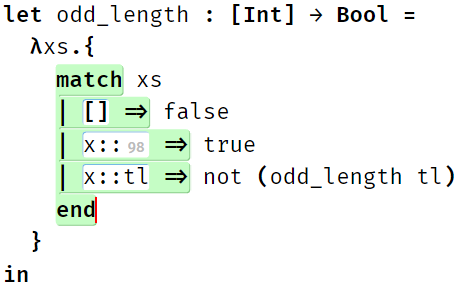
\includegraphics[scale=0.45]{imgs/exhaustive.png}}%
	\subcaptionbox{Indeterminately Exhaustive\label{fig:may-exhaustive}}{
		\raisebox{\dimexpr\ht3-\height}{
			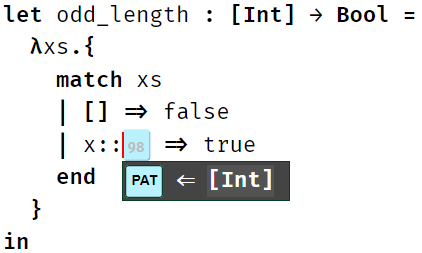
\includegraphics[scale=0.45,valign=t]{imgs/maybe_exhaustive.png}%
			\vphantom{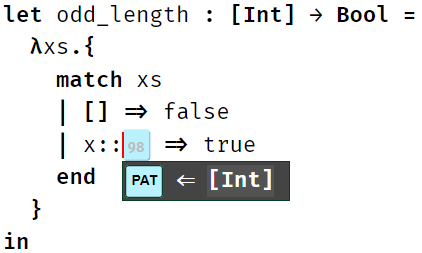
\includegraphics[scale=0.45,valign=t]{imgs/maybe_exhaustive.png}}
		}
	}
	\hfil
	\subcaptionbox{Necessarily Inexhaustive\label{fig:not-exhaustive}}{
		\raisebox{\dimexpr\ht3-\height}{
			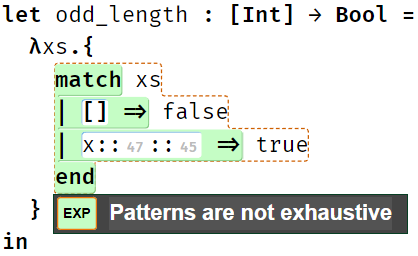
\includegraphics[scale=0.45,valign=t]{imgs/not_exhaustive.png}%
			\vphantom{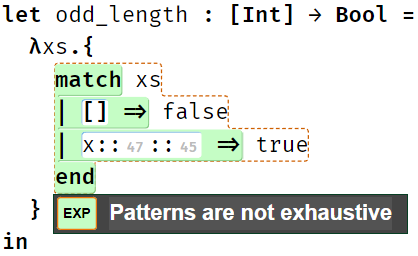
\includegraphics[scale=0.45,valign=t]{imgs/not_exhaustive.png}}
		}
	}
	\hfil
	\subcaptionbox{Necessarily Exhaustive\label{fig:must-exhaustive}}{
		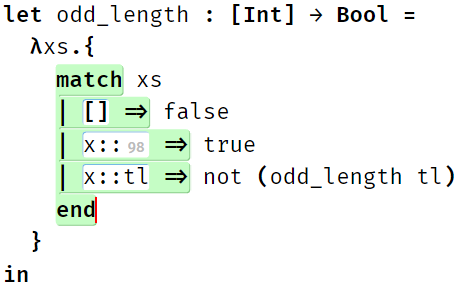
\includegraphics[scale=0.45,valign=t]{imgs/exhaustive.png}
	}
	\caption{Exhaustiveness Checking with Pattern Holes}
	\label{fig:exhaustiveness}
\end{figure}

Explicitly, assume the editor state is as in \autoref{fig:may-exhaustive}. The \li{match} expression contains two rules, the first with an empty list pattern \li{[]}, and the second with a cons cell pattern \li{::} with a variable \li{x} at the head and a pattern hole at the tail. The cursor is placed over the pattern hole, and Hazel is able to infer the type of the pattern as \li{[Int]} from the surrounding context, presenting this information to the user. Should we consider such an expression to be exhaustive? If the user fills the pattern hole with a variable \li{xs}, then the \li{match} is indeed exhaustive: any empty list matches the first pattern, and any non-empty list matches the second pattern. However, if the user instead fills the hole with, say, \li{[]} or \li{y::tl}, then a list with three elements would fail to match any pattern. Thus, without further hole-filling, we can only soundly state that the \li{match} is \emph{indeterminately exhaustive}.

While we cannot guarantee exhaustiveness in \autoref{fig:may-exhaustive}, such indeterminacy does not necessarily reflect an error on the user's part. Instead, they may simply be in the middle of on-going editing, working towards what will soon become an exhaustive expression. To avoid distracting the user with unnecessary information in such a case, in Hazel, we choose not to alert the user of indeterminate exhaustiveness. Instead, we only report an error when, regardless of hole fillings, the expression is always inexhaustive. We say such a \li{match} is \emph{necessarily inexhaustive}, and \autoref{fig:not-exhaustive} provides an illustrative example. The first given rule given only matches the empty list, and the second rule only possibly matches lists with at least two elements, with this holding regardless of the choice of hole-fillings. Thus, in any hole filling, a one element list such as \li{1 :: []} will not match any of the given patterns, and correspondingly, we display an error to the user. Note that the entire \li{match} expression is also resultingly placed within a non-empty hole. This is necessary to prevent evaluation from getting "stuck" when the scrutinee witnesses the inexhaustiveness.

Finally, even with the presence of pattern holes, there are still cases where we can in fact guarantee exhaustiveness. Considering \autoref{fig:must-exhaustive}, the first and third patterns together already cover all appropriately typed expressions. Thus, regardless of how the pattern hole in the second rule is filled, the \li{match} expression as a whole will always be exhaustive, i.e. it is \emph{necessarily exhaustive}. Note that we do not make a visual distinction between necessarily exhaustive and indeterminately exhaustive expressions, again because such information is more likely to be distracting than useful to the user. However, the semantic distinction is interesting to note, and it may be of use to future editor services designed around such holes. 

\subsection{Redundancy Checking with Pattern Holes}\label{sec:redundancy}
From a certain point of view, exhaustiveness checking guarantees a notion of \emph{sufficiency} - that the patterns in a \li{match} expression are sufficient to cover all possible values of the scrutinee's type. Redundancy checking, on the other hand, guarantees a notion of \emph{necessity} - that all the patterns in a \li{match} expressions are in fact required in that none is fully subsumed by other patterns earlier in the sequence. Explicitly, we say that a pattern $p$ in a \li{match} expression is redundant if, for every value $e$ of the scrutinee's type matching $p$, necessarily $e$ also matches some pattern $p^\prime$ preceding $p$ in the sequence of rules. Because a \li{match} expression considers rules one-by-one from the top down, a rule with a redundant pattern will be an unreachable code path. 

As the reader should now anticipate, including pattern holes again requires us to reason conservatively about all possible hole-fillings, thereby introducing indeterminacy into our analysis. That is, a pattern may be either \emph{necessarily redundant}, \emph{necessarily irredundant}, or \emph{indeterminately irredundant} due to the presence of expression or pattern holes. Similarly to how we handled exhaustiveness checking, we again only alert the user in cases where an error is guaranteed, i.e. when a rule is necessarily redundant.

\begin{figure}
	\centering
	\subcaptionbox{Necessarily Irredundant (first two patterns) + Indeterminately Irredundant (third pattern)\label{fig:may-redundant}}{
		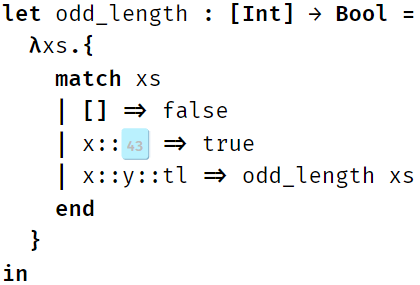
\includegraphics[scale=0.5,valign=t]{imgs/maybe_redundant.png}%
		\vphantom{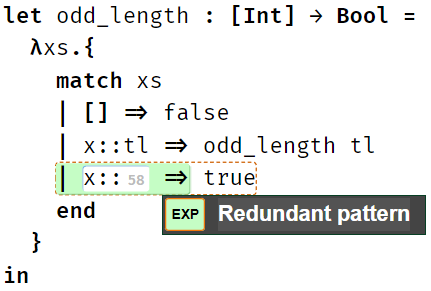
\includegraphics[scale=0.5,valign=t]{imgs/redundant.png}}
	} 
	\hfil
	\subcaptionbox{Necessarily Redundant (third pattern) \label{fig:must-redundant}}{
		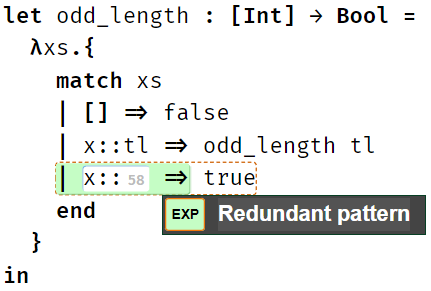
\includegraphics[scale=0.5,valign=t]{imgs/redundant.png}
	}%
	\caption{Redundancy Checking with Pattern Holes}
	\label{fig:redundancy}
\end{figure}

\autoref{fig:redundancy} concretely demonstrates all of these possibilities, continuing with our running example of an \li{odd_length} function. In the editor state in \autoref{fig:may-redundant}, there is a pattern hole in the second pattern. Depending on how this pattern hole is filled, the third pattern can be made either redundant or irredundant. Explicitly, if we filled the hole with the empty list \li{[]}, then the third pattern is the only one which matching lists with more than one element, so it is irredundant. If instead we filled the hole with \li{y::tl}, then the second pattern is in fact the same as third pattern, and obviously subsumes it. Thus, we can only soundly state that the third pattern is indeterminately irredundant.

For the second pattern itself, despite containing a pattern hole, we can still deem it necessarily irredundant. The only pattern proceeding it is an empty list \li{[]}, while the second pattern only matches non-empty lists regardless of hole filling. Thus, no hole filling allows the second pattern to be made redundant by the first. Note that, vacuously, the first pattern is also necessarily irredundant - it cannot be subsumed by previous rules because there are no previous rules. Similarly, the first pattern of any \li{match} expression is necessarily irredundant, except in the case when the scrutinee's type has no values at all (e.g. is of \li{void} type). In this case, all rules are necessarily redundant.

Finally, the editor state in \autoref{fig:must-redundant} showcases a necessarily redundant pattern. Explicitly, regardless of the choice of hole filling, the third pattern can only be matched by a non-empty list. However, the second pattern already matches all such non-empty lists. Thus, the third pattern is necessarily redundant, and correspondingly, we report an error to the user. Note that, in this particular case, the first two rules are already exhaustive, so any pattern we could possibly place in the third rule will be necessarily redundant. More generally, stating that a pattern $p$ is redundant is equivalent to stating that the preceding patterns exhaustively cover all values matching $p$. As we will explore in more detail in \autoref{sec:analyses}, this enables us to reduce the problem of redundancy checking to that of exhaustiveness checking.

\section{Peanut: A Typed Pattern Hole Calculus}\label{sec:peanut}
We now formalize the high-level discussion described in \autoref{sec:pattern-matching}. While all of our work has been implemented into the full Hazel system, for ease of presentation, we distill our contribution into a bare-bones typed lambda calculus called Peanut. The core of our calculus is based upon the Hazelnut Live internal language \cite{DBLP:journals/pacmpl/OmarVCH19}, but extended to include pattern holes. We develop a dynamic semantics which allows live evaluation as discussed in \autoref{sec:live-eval}, and additionally, present a static semantic guaranteeing exhaustiveness and irredundancy as discussed in \autoref{sec:exhaustiveness} and \autoref{sec:redundancy}. 

We begin in \autoref{sec:syntax} by presenting the syntax of our calculus. In \autoref{sec:dynamics}, we then provide a small-step dynamic semantics with support for evaluating incomplete programs. In \autoref{sec:constraints}, \autoref{sec:statics}, and \autoref{sec:analyses}, we give the corresponding static semantics as a system of type assignment, making use a constraint language to reason about exhaustiveness and irredundancy. We defer discussion of decidability and implementation until \autoref{sec:decidability}.

\subsection{Syntax}\label{sec:syntax}
% !TeX root = presentation.tex

\begin{figure}[ht]
    \centering
    \begin{minipage}{.5\linewidth}
  $\arraycolsep=4pt\begin{array}{lll}
    e & ::= &
      x ~\vert~
      \hnum{n} \\
      & ~\vert~ &
      \hlam{x}{\tau}{e} ~\vert~
      \hap{e_1}{e_2} \\
      & ~\vert~ &
      \hpair{e_1}{e_2} ~\vert~
      \hfst{e} ~\vert~ \hsnd{e} \\
      & ~\vert~ &
      \hinl{\tau}{e} ~\vert~
      \hinr{\tau}{e} \\
      & ~\vert~ &
      \hmatch{e}{\hat{rs}} \\
      & ~\vert~ &
      \hehole{u} ~\vert~
      \hhole{e}{u} \\
    \end{array}$
    \end{minipage}%
    \begin{minipage}{.5\linewidth}
  $\arraycolsep=4pt\begin{array}{lll}
    \tau & ::= &
      \tnum ~\vert~
      \tarr{\tau_1}{\tau_2}\\
      & ~\vert~ &
      \tprod{\tau_1}{\tau_2} ~\vert~
      \tsum{\tau_1}{\tau_2} \\
    \hat{rs} & ::= &
      \zrulsP{rs}{r}{rs} \\
    rs & ::= &
      \cdot ~\vert~ \hrulesP{r}{rs'} \\
    r & ::= &
      \hrul{p}{e} \\
    p & ::= &
      x ~\vert~
      \_ ~\vert~
      \hnum{n} ~\vert~
      \hpair{p_1}{p_2} \\
      & ~\vert~ &
      \hinlp{p} ~\vert~
      \hinrp{p} \\
      & ~\vert~ &
      \heholep{w} ~\vert~
      \hholep{p}{w}{\tau}
    \end{array}$
    \end{minipage}
\end{figure}

% !TeX root = thesis.tex

\begin{figure}[ht]

\judgbox{\rmpointer{\zrules} = rs}
        {$rs$ can be obtained by erasing the pointer from $\zrules$}
\begin{align*}
  \rmpointer{\zruls{\cdot}{r}{rs}} &= \hrules{r}{rs} \\
  \rmpointer{\zruls{\hrulesP{r'}{rs'}}{r}{rs}} &= \hrules{r'}{\rmpointer{\zruls{rs'}{r}{rs}}}
\end{align*}

\caption{Rule Pointer Erasure}
\label{fig:pointer-eraser}
\end{figure}


Figure \ref{fig:syntax} presents the syntax of Peanut. Peanut closely mirrors the internal language of Hazelnut Live \cite{DBLP:journals/pacmpl/OmarVCH19}, a typed lambda calculus with expression holes which provides the base of the Hazel system. For ease of presentation, we attempt to include only those forms necessary to have a rich discussion of pattern matching. Resultingly, we remove most of the machinery related to gradual typing \cite{DBLP:conf/snapl/SiekVCB15}, but such an extension is fairly straightforward to implement. Most of the forms are standard, and we follow their formulations outlined in \cite{Harper2012}. 

Unsurprisingly, we include lambda functions and function application. We choose natural numbers as our base type. In order to create interesting expressions to pattern match on, we also allow the formation of binary sum and binary product types. Correspondingly, we include pairs, projection operators, and left and right injections. (Note that pattern matching generally negates the need for explicit projections operators, but we include such forms here for reasons discussed later.) To simplify our type assignment system, we also require injections and functions to have explicit type annotations. Such annotations are fairly innocuous, as Peanut represents an internal language, so if desired, annotations can always be inserted during elaboration. Finally, we include the main forms of interest: holes, patterns, and match expressions.

As discussed in \autoref{sec:intro}, holes come in two variants. Empty expression holes are written $\hehole{u}$ and indicate missing syntactic pieces, while non-empty holes expression holes are written $\hhole{e}{u}$ and act as a membrane around a type inconsistency at the expression $e$. Analogously, empty pattern holes are written $\heholep{w}$ and indicate missing sub-terms of a pattern, while non-empty pattern holes are written $\hholep{p}{w}{\tau}$ and surround a type-inconsistency, with $\tau$ recording the type of $p$. Here, the labels $u$ and $w$ are identifiers for the corresponding hole. As Peanut represents an internal language, distinct identifiers should correspond to distinct holes in the original program. However, as evaluation can lead to holes being replicated during substitution, we do not enforce a uniqueness constraint within Peanut itself.

Outside of holes, patterns also include a form corresponding to each constructor for values, variables, and a wildcard pattern $(\_)$. Semantically, the wildcard is matched by any expression, allowing the user to indicate a default case. Match expressions $\hmatch{e}{\zrules}$ then consist of a scrutinee $e$ and a list of rules $\zrules$. As we wish to allow live evaluation, we must be able to represent intermediate execution states of the match expression. Correspondingly, the list $\zrules$ is zippered \cite{DBLP:journals/jfp/Huet97}, effectively containing a pointer to the current rule under consideration. Syntactically, this is given by a triple, $\zruls{rs_{pre}}{r}{rs_{post}}$, with a prefix list of rules already considered, $rs_{pre}$, the current rule, $r$, and a suffix list of rules yet to be considered, $rs_{post}$ . We can erase this pointer through the pointer erasure operator, $\rmpointer{\zrules}$, as defined in \autoref{fig:pointer-eraser}, yielding an unzippered list. Each rule is of the form $\hrul{p}{e}$, where $p$ is a pattern and $er$ is the corresponding branch expression. 

\subsection{Dynamic Semantics}\label{sec:dynamics}

% !TeX root = thesis.tex

\begin{figure}[h]

\judgbox{\htrans{e}{e'}}{$e$ takes a step to $e'$}

\begin{mathpar}
\Infer{\ITHole}{
 \htrans{e}{e'}
}{
 \htrans{\hhole{e}{u}}{\hhole{e'}{u}}
}

\Infer{\ITApFun}{
 \htrans{e_1}{e_1'}
}{
 \htrans{\hap{e_1}{e_2}}{\hap{e_1'}{e_2}}
}

\Infer{\ITApArg}{
 \isFinal{e_1} \\
 \htrans{e_2}{e_2'}
}{
 \htrans{\hap{e_1}{e_2}}{\hap{e_1}{e_2'}}
}

\Infer{\ITAp}{
 \isFinal{e_2}
}{
 \hap{\hlam{x}{\tau}{e_1}}{e_2} \mapsto
   [e_2/x]e_1
}

\Infer{\ITPairL}{
 \htrans{e_1}{e_1'}
}{
 \htrans{\hpair{e_1}{e_2}}{\hpair{e_1'}{e_2}}
}

\Infer{\ITPairR}{
 \isFinal{e_1} \\
 \htrans{e_2}{e_2'}
}{
 \htrans{\hpair{e_1}{e_2}}{\hpair{e_1}{e_2'}}
}

\Infer{\ITFst}{
 \htrans{e_1}{e_1'}
}{
 \htrans{\hfst{e_1}}{\hfst{e_1'}}
}

\Infer{\ITSnd}{
 \htrans{e_1}{e_1'}
}{
 \htrans{\hsnd{e_1}}{\hsnd{e_1'}}
}

\Infer{\ITFstPair}{
 \isFinal{\hpair{e_1}{e_2}}
}{
 \htrans{\hfst{\hpair{e_1}{e_2}}}{e_1}
}

\Infer{\ITSndPair}{
 \isFinal{\hpair{e_1}{e_2}}
}{
 \htrans{\hsnd{\hpair{e_1}{e_2}}}{e_2}
}

\Infer{\ITInl}{
 \htrans{e}{e'}
}{
 \htrans{\hinl{\tau}{e}}{\hinl{\tau}{e'}}
}

\Infer{\ITInr}{
 \htrans{e}{e'}
}{
 \htrans{\hinr{\tau}{e}}{\hinr{\tau}{e'}}
}

\Infer{\ITExpMatch}{
  \htrans{e}{e'}
}{
  \htrans{\hmatch{e}{\zrules}}{\hmatch{e'}{\zrules}}
}

\Infer{\ITSuccMatch}{
  \isFinal{e} \\
  \hpatmatch{e}{p_r}{\theta}
}{
  \htrans{
    \hmatch{e}{\zruls{rs_{pre}}{\hrulP{p_r}{e_r}}{rs_{post}}}
  }{
    [\theta](e_r)
  }
}

\Infer{\ITFailMatch}{
  \isFinal{e} \\
  \hnotmatch{e}{p_r}
}{
  \htrans{
    \hmatch{e}{\zruls{rs}{\hrulP{p_r}{e_r}}{\hrulesP{r'}{rs'}}}
  }{
    \hmatch{e}{
      \zruls{
        \rmpointer{\zruls{rs}{\hrulP{p_r}{e_r}}{\cdot}}
      }{r'}{rs'}
    }
  }
}
\end{mathpar}

\caption{Stepping}
\label{fig:step}
\end{figure}

% !TeX root = thesis.tex

\begin{figure}[th]

\begin{minipage}{.45\linewidth}
\judgbox{\isVal{e}}{$e$ is a value}

\begin{mathpar}
\Infer{\VNum}{ }{
  \isVal{\hnum{n}}
}

\Infer{\VLam}{ }{
  \isVal{\hlam{x}{\tau}{e}}
}

\Infer{\VPair}{
  \isVal{e_1} \\
  \isVal{e_2}
}{
  \isVal{\hpair{e_1}{e_2}}
}

\Infer{\VInl}{
  \isVal{e}
}{
  \isVal{\hinl{\tau}{e}}
}

\Infer{\VInr}{
  \isVal{e}
}{
  \isVal{\hinr{\tau}{e}}
}
\end{mathpar}
\end{minipage}%
\begin{minipage}{.45\linewidth}
\judgbox{\isIndet{e}}{$e$ is indeterminate}

\begin{mathpar}
...

\Infer{\IEHole}{ }{
 \isIndet{\hehole{u}}
}

\Infer{\IHole}{
 \isFinal{e}
}{
 \isIndet{\hhole{e}{u}}
}

\Infer{\IAp}{
 \isIndet{e_1} \\ \isFinal{e_2}
}{
 \isIndet{\hap{e_1}{e_2}}
}

\Infer{\IPairL}{
 \isIndet{e_1} \\ \isVal{e_2}
}{
 \isIndet{\hpair{e_1}{e_2}}
}

\Infer{\IPairR}{
 \isVal{e_1} \\ \isIndet{e_2}
}{
 \isIndet{\hpair{e_1}{e_2}}
}

\Infer{\IPair}{
 \isIndet{e_1} \\ \isIndet{e_2}
}{
 \isIndet{\hpair{e_1}{e_2}}
}

\Infer{\IFst}{
 \isIndet{e} \\ e \neq \hpair{e_1}{e_2}
}{
 \isIndet{\hfst{e}}
}

\Infer{\ISnd}{
 \isIndet{e} \\ e \neq \hpair{e_1}{e_2}
}{
 \isIndet{\hsnd{e}}
}

\Infer{\IInl}{
 \isIndet{e}
}{
 \isIndet{\hinl{\tau}{e}}
}

\Infer{\IInr}{
 \isIndet{e}
}{
 \isIndet{\hinr{\tau}{e}}
}

\Infer{\IMatch}{
  \isFinal{e} \\
  \hmaymatch{e}{p_r}
}{
  \isIndet{
    \hmatch{e}{\zruls{rs_{pre}}{\hrulP{p_r}{e_r}}{rs_{post}}}
  }
}
\end{mathpar}
\judgbox{\isFinal{e}}{$e$ is final}
\begin{mathpar}
\Infer{\FVal}{
  \isVal{e}
}{
  \isFinal{e}
}

\Infer{\FIndet}{
  \isIndet{e}
}{
  \isFinal{e}
}
\end{mathpar}

\end{minipage}

  \caption{Final expressions}
  \label{fig:final}
\end{figure}


Dynamically, Peanut seeks to extend Hazelnut Live \cite{DBLP:journals/pacmpl/OmarVCH19} while maintaining the ability to evaluate "around" expressions with holes. That is, upon encountering a hole, Peanut should delay its evaluation as long as possible, then proceed to take all other evaluation steps which do not rely on the eventual contents of the hole. For all non-pattern matching forms, our rules correspond exactly to the rules of Hazelnut Live, albeit, formulated as a small-step operational semantics rather than a contextual one. \autoref{fig:step} displays this stepping judgement $\htrans{e}{e'}$, indicating that evaluating an expression $e$ one step yields the expression $e^\prime$.

To begin, consider how one typically evaluates, say, a function application $\hap{e}{e^\prime}$ in a strict language without holes. Initially, the function $e$ is stepped as far as possible, continuing until it is reduced to a value. Next, evaluation steps the argument $e^\prime$, again continuing until it is reduced to a value. Once all these reductions have occurred, only then is an actual substitution applied. Notably, the key ingredient to this process is the ability to detect when an expression has been reduced "as far as possible", or equivalently, when an expression has been reduced to a value. 

In the presence of pattern and expression holes, evaluation proceeds in much the same way. \autoref{fig:final} defines a judgement $\isFinal{e}$ indicating when an expression $e$ is \emph{final}, i.e when no further evaluation steps can occur. The rules \ITApFun, \ITApArg, and \ITAp are then the same as we described in our example. Crucially, however, holes extend the notion of finality to include not just values, but \emph{indeterminate} forms as well. That is, there are terms which have indeed been reduced as far as possible, but they still contain holes in the end result, and they will require further evaluation if such holes are filled at a later point in time. We differentiate between these cases with the judgement $\isVal{e}$, characterizing values, and the judgement $\isIndet{e}$, characterizing indeterminate expressions. Correspondingly, the $\isFinal{e}$ judgement is given as a disjunction of these two cases.

For Peanut, the main task is to describe the behavior of a match expression $\hmatch{e}{\zrules}$. First, as described by \ITExpMatch, we step the scrutinee $e$, eventually yielding either a value or indeterminate form. Once $e$ is final, we then proceed to pattern match, comparing $e$ to each pattern sequentially from the top down. If $e$ indeed matches a pattern, then we step to the corresponding branch expression as in the conclusion of \ITSuccMatch. Instead, if $e$ does not match the pattern as in \ITFailMatch, then we move to consider the next rule, using the pointer erasure operator of \autoref{fig:pointer-eraser} to increment the zipper. Note that, per our previous discussion, an expression may also indeterminately match a pattern. The \IMatch rule in the $\isIndet{e}$ judgement covers this case, indicating that we cannot safely proceed past an indeterminate pattern match, leading to the entire match expression being indeterminate without further hole-filling.

Our stepping and finality judgements indeed cover all possible cases. The following theorem states this, combining progress and determinism. Here, the judgement $\hexptyp{\cdot}{\Delta}{e}{\tau}$ indicates that $e$ is a closed term of type $\tau$, as discussed further in \autoref{sec:statics} when presenting Peanut's static semantics.

\begin{theorem}[Deterministic Progress]
	\label{theorem:determinism}
	If $\hexptyp{\cdot}{\Delta}{e}{\tau}$ then exactly one of the following holds
	\begin{enumerate}
		\item $\isVal{e}$
		\item $\isIndet{e}$
		\item $\htrans{e}{e'}$ for some unique $e'$
	\end{enumerate}
\end{theorem}

Essential to the aforementioned rules are the judgements determining whether an expression $e$ must match, must not match, or indeterminately matches a pattern $p$. \autoref{fig:patmatch} presents these three cases. First, the judgement $\hpatmatch{e}{p}{\theta}$ indicates that $e$ successfully matches $p$, emitting a series of corresponding substitutions $\theta$ for the variables bound in $p$. Next, the judgement $\hnotmatch{e}{p}$ indicates that $e$ does not match $p$. Finally, the judgement $\hmaymatch{e}{p}$ indicates that $e$ indeterminately matches $p$ depending on the eventual contents of holes in $e$ or $p$. These judgements correspond respectively to the rules \ITSuccMatch, \ITFailMatch, and \IMatch discussed above, appearing as a premise in each.

As desired, these three matching judgements are exclusive and cover all possible cases. Again, the judgement $\hexptyp{\cdot}{\Delta}{e}{\tau}$ states that $e$ is a closed term of type $\tau$, while the judgement $\hpattyp{p}{\tau}{\Gamma}{\Delta}$ indicates that we can also assign the type $\tau$ to our pattern $p$. Note that because of the correspondence between these matching judgements and the semantics of the match expression, the following lemma encapsulates the majority of the work required to prove $\autoref{theorem:determinism}$.

\begin{lemma}[Matching Determinism]
	\label{lemma:match-determinism}
	If $\isFinal{e}$ and $\hexptyp{\cdot}{\Delta}{e}{\tau}$ and $\hpattyp{p}{\tau}{\Gamma}{\Delta}$ then exactly one of the following holds
	\begin{enumerate}
		\item $\hpatmatch{e}{p}{\theta}$ for some $\theta$
		\item $\hmaymatch{e}{p}$
		\item $\hnotmatch{e}{p}$
	\end{enumerate}
\end{lemma}

% !TeX root = thesis.tex

\begin{figure}[h!]

\judgbox{
  \hpatmatch{e}{p}{\theta}
}{
  $e$ matches $p$, emitting $\theta$
}

\begin{mathpar}
\Infer{\MVar}{ }{
  \hpatmatch{e}{x}{e / x}
}

\Infer{\MWild}{ }{
  \hpatmatch{e}{\_}{\cdot}
}

\Infer{\MNum}{ }{
  \hpatmatch{\hnum{n}}{\hnum{n}}{\cdot}
}

\Infer{\MPair}{
  \hpatmatch{e_1}{p_1}{\theta_1} \\
  \hpatmatch{e_2}{p_2}{\theta_2}
}{
  \hpatmatch{\hpair{e_1}{e_2}}{\hpair{p_1}{p_2}}{\theta_1 \uplus \theta_2}
}

\Infer{\MInl}{
  \hpatmatch{e}{p}{\theta}
}{
  \hpatmatch{\hinl{\tau}{e}}{\hinlp{p}}{\theta}
}

\Infer{\MInr}{
  \hpatmatch{e}{p}{\theta}
}{
  \hpatmatch{\hinr{\tau}{e}}{\hinrp{p}}{\theta}
}

\Infer{\MNotIntroPair}{
  \notIntro{e} \\
  \hpatmatch{\hfst{e}}{p_1}{\theta_1} \\
  \hpatmatch{\hsnd{e}}{p_2}{\theta_2}
}{
  \hpatmatch{e}{\hpair{p_1}{p_2}}{\theta_1 \uplus \theta_2}
}
\end{mathpar}

\judgbox{
  \hnotmatch{e}{p}
}{
  $e$ does not match $p$
}

\begin{mathpar}

\Infer{\NMNum}{
  n_1 \neq n_2
}{
  \hnotmatch{\hnum{n_1}}{\hnum{n_2}}
}

\Infer{\NMPairL}{
  \hnotmatch{e_1}{p_1}
}{
  \hnotmatch{\hpair{e_1}{e_2}}{\hpair{p_1}{p_2}}
}

\Infer{\NMPairR}{
  \hnotmatch{e_2}{p_2}
}{
  \hnotmatch{\hpair{e_1}{e_2}}{\hpair{p_1}{p_2}}
}

\Infer{\NMConfL}{ }{
  \hnotmatch{\hinr{\tau}{e}}{\hinlp{p}}
}

\Infer{\NMConfR}{ }{
  \hnotmatch{\hinl{\tau}{e}}{\hinrp{p}}
}

\Infer{\NMInl}{
  \hnotmatch{e}{p}
}{
  \hnotmatch{\hinl{\tau}{e}}{\hinlp{p}}
}

\Infer{\NMInr}{
  \hnotmatch{e}{p}
}{
  \hnotmatch{\hinr{\tau}{e}}{\hinrp{p}}
}
\end{mathpar}

\judgbox{
  \hmaymatch{e}{p}
}{
  $e$ indeterminately matches $p$
}

\begin{mathpar}
\Infer{\MMEHole}{ }{
  \hmaymatch{e}{\heholep{w}}
}

\Infer{\MMHole}{ }{
  \hmaymatch{e}{\hholep{p}{w}{\tau}}
}
\\
\Infer{\MMNotIntro}{
  \notIntro{e} \\
  \refutable{p}
}{
  \hmaymatch{e}{p}
}

\Infer{\MMPairL}{
  \hmaymatch{e_1}{p_1} \\
  \hpatmatch{e_2}{p_2}{\theta_2}
}{
  \hmaymatch{\hpair{e_1}{e_2}}{\hpair{p_1}{p_2}}
}

\Infer{\MMPairR}{
  \hpatmatch{e_1}{p_1}{\theta_1} \\
  \hmaymatch{e_2}{p_2}
}{
  \hmaymatch{\hpair{e_1}{e_2}}{\hpair{p_1}{p_2}}
}

\Infer{\MMPair}{
  \hmaymatch{e_1}{p_1} \\
  \hmaymatch{e_2}{p_2}
}{
  \hmaymatch{\hpair{e_1}{e_2}}{\hpair{p_1}{p_2}}
}

\Infer{\MMInl}{
  \hmaymatch{e}{p}
}{
  \hmaymatch{\hinl{\tau}{e}}{\hinlp{p}}
}

\Infer{\MMInr}{
  \hmaymatch{e}{p}
}{
  \hmaymatch{\hinr{\tau}{e}}{\hinrp{p}}
}
\end{mathpar}

\caption{Three possible outcomes of pattern matching}
\label{fig:patmatch}
\end{figure}

% !TEX root = thesis.tex

\begin{figure}[ht]
\judgbox{
  \notIntro{e}
}{
  $e$ cannot be a value syntactically
}

\begin{mathpar}
\Infer{NVEHole}{ }{
  \notIntro{\hehole{u}}
}

\Infer{NVHole}{ }{
  \notIntro{\hhole{e}{u}}
}

\Infer{NVAp}{ }{
  \notIntro{\hap{e_1}{e_2}}
}

\Infer{NVMatch}{ }{
  \notIntro{\hmatch{e}{\zrules}}
}

\Infer{NVFst}{ }{
  \notIntro{\hfst{e}}
}

\Infer{NVSnd}{ }{
  \notIntro{\hsnd{e}}
}
\end{mathpar}

  \caption{Expressions that are syntactically not values}
  \label{fig:notintro}
\end{figure}

% !TeX root = thesis.tex

\begin{figure}[hb!]
\judgbox{
  \refutable{p}
}{$p$ is refutable}

\begin{mathpar}
\Infer{\RNum}{ }{
  \refutable{\hnum{n}}
}

\Infer{\REHole}{ }{
  \refutable{\heholep{w}}
}

\Infer{\RHole}{ }{
  \refutable{\hholep{p}{w}{\tau}}
}

\Infer{\RInl}{ }{
  \refutable{\hinlp{p}}
}

\Infer{\RInr}{ }{
  \refutable{\hinrp{p}}
}

\Infer{\RPairL}{
  \refutable{p_1}
}{
  \refutable{\hpair{p_1}{p_2}}
}

\Infer{\RPairR}{
  \refutable{p_2}
}{
  \refutable{\hpair{p_1}{p_2}}
}
\end{mathpar}
\caption{Refutable Patterns}
\label{fig:refutable}
\end{figure}


Let us now explore these pattern matching judgements in more depth, considering matching an expression $e$ against a pattern $p$. Note that semantics of our expression guarantees that we only perform pattern matching on well-typed and final scrutinees (per the inclusion of $\isFinal{e}$ as a premise to \ITSuccMatch and \ITFailMatch). Throughout this discussion, we then assume $e$ is final and that $e$ and $p$ are of the same type.

If we ignore cases of indeterminacy, most of the rules are fairly straightforward. For the judgement $\hpatmatch{e}{p}{\theta}$, each rule specifies that $e$ and $p$ have the same outermost constructor, and that their corresponding subterms match inductively. Conversely, the rules for $\hnotmatch{e}{p}$ identify a cases where either the outermost constructors of $e$ and $p$ mismatch (e.g. \NMInl and \NMInr), or where their outermost constructors agree, but some corresponding subterm inductively fails to match (e.g. \NMPairL and \NMPairR).

To reason about indeterminacy, however, we require a few auxillary judgements. As our scrutinee is final, it will be indeterminate if and only if it is not a value. \autoref{fig:notintro} defines a judgement $\notIntro{e}$ which characterizes this case, syntactically analyzing the outermost constructor of $e$ to determine that it cannot be a value. Note that an indeterminate $e$ will be further evaluated after hole filling, so correspondingly, our rules should treat such an $e$ as opaque, never inspecting any of its subterms. However, even with this restriction, there are still cases where $e$ must match a pattern $p$. That is, a pattern $p$ could be irrefutable in the sense that it must be matched by all expressions of the same type, say, if it is a variable \li{x} or wildcard $\_$. Correspondingly, \autoref{fig:refutable} defines a judgement $\refutable{p}$ indicating that $p$ is not irrefutable, i.e. there is some hole filling which allows at least one expression to fail to match $p$.

Together, the combinations of these judgements allows us to identify all indeterminate matches. The rule \MMNotIntro gives that a match is indeterminate whenever $e$ is indeterminate and $p$ is not irrefutable. The rules \MMEHole and \MMHole state that directly matching against a hole will always be indeterminate. All other indeterminacy arises inductively from some subterms indeterminately matching. Conversely, even in the case when $e$ is indeterminate, we wish to have $e$ match an irrefutable pattern $p$. The rules \MVar and \MWild give two explicit cases of this. In \MNotIntroPair, the irrefutability is implicit - a term $\hfst{e}$ or $\hsnd{e}$ can only match an irrefutable pattern, but we explicitly derive the matching judgements in order to emit appropriate substitutions

\subsection{Match Constraint Language}\label{sec:constraints}
With the dynamic semantics of Peanut defined, we now turn to the problem of statically reasoning about the runtime behavior of our programs. In particular, we focus on ensuring exhaustiveness and redundancy of match expressions. Towards this end, we extend an idea outlined in \cite{Harper2012} by introducing a \emph{match constraint language}. Intuitively, such a language encodes the logic of patterns, with each constraint corresponding to the restriction that a pattern puts on those expression matching it. Further, additional constraints are added to allow taking negation, logical and ($\land$), and logical or ($\lor$). In \autoref{sec:statics}, we explicitly describe how constraints are generated by patterns. In \autoref{sec:analyses}, we then describe how constraints enable static reasoning about exhaustiveness and irredundancy.

% !TeX root = presentation.tex

\begin{figure}[ht]
$\arraycolsep=4pt\begin{array}{lll}
\xi & ::= &
  \ctruth ~\vert~
  \cfalsity ~\vert~
  \cunknown ~\vert~
  \cnum{n} ~\vert~
  \cnotnum{n} ~\vert~
  \cand{\xi_1}{\xi_2} ~\vert~
  \cor{\xi_1}{\xi_2} ~\vert~
  \cinl{\xi} ~\vert~
  \cinr{\xi} ~\vert~
  \cpair{\xi_1}{\xi_2}
\end{array}$
\end{figure}


The syntax of the constraint language is displayed in \autoref{fig:constraint}. Note that each pattern indeed has a corresponding constraint of the same syntactic form. The only exception here is that variables and wildcards both map to the truth constraint ($\ctruth$), as they are both matched by any expression. We specify that a constraint $\xi$ restricts expressions of type $\tau$ with the constraint type assignment judgement $\ctyp{\xi}{\tau}$. Ignoring indeterminacy and $\cunknown$ for now, one can explicitly model constraints of type $\tau$ as the Boolean algebra formed by subsets of the set of all final expressions of type $\tau$. That is, a constraint $\ctyp{\xi}{\tau}$ can be interpreted as the set of all final expressions of type $\tau$ which \emph{satisfy} $\xi$. Correspondingly, the \emph{dual} of $\xi$ , written $\cdual{\xi}$, is satisfied by all appropriately-typed final expressions not satisfying $\xi$, and thus can be interpreted as the complement of the set identified by $\xi$. The truth constraint $\ctruth$ and falsity constraint $\cfalsity$ are intrepreted as the whole set and the empty set respectively. Up to equivalence, the usual laws of Boolean logic hold, e.g. the dual of $\cdual{\xi}$ should be equivalent to $\xi$.

% !TeX root = thesis.tex

\begin{figure}[!ht]

\judgbox{\csatisfy{e}{\xi}}{$e$ necessarily satisfies $\xi$}

\begin{mathpar}
\Infer{\CSTruth}{ }{
  \csatisfy{e}{\ctruth}
}

\Infer{\CSNum}{ }{
  \csatisfy{\hnum{n}}{\cnum{n}}
}

\Infer{\CSNotNum}{
  n_1 \neq n_2
}{
  \csatisfy{\hnum{n_1}}{\cnotnum{n_2}}
}

\Infer{\CSAnd}{
  \csatisfy{e}{\xi_1} \\
  \csatisfy{e}{\xi_2}
}{
  \csatisfy{e}{\cand{\xi_1}{\xi_2}}
}

\Infer{\CSOrL}{
  \csatisfy{e}{\xi_1}
}{
  \csatisfy{e}{\cor{\xi_1}{\xi_2}}
}

\Infer{\CSOrR}{
  \csatisfy{e}{\xi_2}
}{
  \csatisfy{e}{\cor{\xi_1}{\xi_2}}
}

\Infer{\CSInl}{
  \csatisfy{e_1}{\xi_1}
}{
  \csatisfy{
    \hinl{\tau_2}{e_1}
  }{
    \cinl{\xi_1}
  }
}

\Infer{\CSInr}{
  \csatisfy{e_2}{\xi_2}
}{
  \csatisfy{
    \hinr{\tau_1}{e_2}
  }{
    \cinr{\xi_2}
  }
}

\Infer{\CSPair}{
  \csatisfy{e_1}{\xi_1} \\
  \csatisfy{e_2}{\xi_2}
}{
\csatisfy{\hpair{e_1}{e_2}}{\cpair{\xi_1}{\xi_2}}
}

\Infer{\CSNotIntroPair}{
  \notIntro{e} \\
  \csatisfy{\hfst{e}}{\xi_1} \\
  \csatisfy{\hsnd{e}}{\xi_2}
}{
  \csatisfy{e}{\cpair{\xi_1}{\xi_2}}
}
\end{mathpar}

\judgbox{\cmaysatisfy{e}{\xi}}{$e$ indeterminately satisfy $\xi$}

\begin{mathpar}
\Infer{\CMSUnknown}{ }{
  \cmaysatisfy{e}{\cunknown}
}

\Infer{\CMSNotIntro}{
  \notIntro{e} \\
  \refutable{\xi} \\
  \possible{\xi}
}{
  \cmaysatisfy{e}{\xi}
}

\Infer{\CMSAndL}{
  \cmaysatisfy{e}{\xi_1} \\
  \csatisfy{e}{\xi_2}
}{
  \cmaysatisfy{e}{\cand{\xi_1}{\xi_2}}
}

\Infer{\CMSAndR}{
  \csatisfy{e}{\xi_1} \\
  \cmaysatisfy{e}{\xi_2}
}{
  \cmaysatisfy{e}{\cand{\xi_1}{\xi_2}}
}

\Infer{\CMSAnd}{
  \cmaysatisfy{e}{\xi_1} \\
  \cmaysatisfy{e}{\xi_2}
}{
  \cmaysatisfy{e}{\cand{\xi_1}{\xi_2}}
}

\Infer{\CMSOrL}{
  \cmaysatisfy{e}{\xi_1} \\
  \cnotsatisfy{e}{\xi_2}
}{
  \cmaysatisfy{e}{\cor{\xi_1}{\xi_2}}
}

\Infer{\CMSOrR}{
  \cnotsatisfy{e}{\xi_1} \\
  \cmaysatisfy{e}{\xi_2}
}{
  \cmaysatisfy{e}{\cor{\xi_1}{\xi_2}}
}

\Infer{\CMSInl}{
  \cmaysatisfy{e_1}{\xi_1}
}{
  \cmaysatisfy{
    \hinl{\tau_2}{e_1}
  }{
    \cinl{\xi_1}
  }
}

\Infer{\CMSInr}{
  \cmaysatisfy{e_2}{\xi_2}
}{
  \cmaysatisfy{
    \hinr{\tau_1}{e_2}
  }{
    \cinr{\xi_2}
  }
}

\Infer{\CMSPairL}{
  \cmaysatisfy{e_1}{\xi_1} \\
  \csatisfy{e_2}{\xi_2}
}{
  \cmaysatisfy{\hpair{e_1}{e_2}}{\cpair{\xi_1}{\xi_2}}
}

\Infer{\CMSPairR}{
  \csatisfy{e_1}{\xi_1} \\
  \cmaysatisfy{e_2}{\xi_2}
}{
  \cmaysatisfy{\hpair{e_1}{e_2}}{\cpair{\xi_1}{\xi_2}}
}

\Infer{\CMSPair}{
  \cmaysatisfy{e_1}{\xi_1} \\
  \cmaysatisfy{e_2}{\xi_2}
}{
  \cmaysatisfy{\hpair{e_1}{e_2}}{\cpair{\xi_1}{\xi_2}}
}
\end{mathpar}

\judgbox{\csatisfyormay{e}{\xi}}{$e$ necessarily or indeterminately satisfy $\xi$}

\begin{mathpar}
\Infer{\CSMSMay}{
  \cmaysatisfy{e}{\xi}
}{
  \csatisfyormay{e}{\xi}
}

\Infer{\CSMSSat}{
  \csatisfy{e}{\xi}
}{
  \csatisfyormay{e}{\xi}
}
\end{mathpar}

  \caption{Satisfaction}
  \label{fig:satisfy}
\end{figure}


Just as we introduced pattern holes into patterns, we include an unknown constraint $(\cunknown)$ in our constraint language to represent indeterminacy. Correspondingly, we have analogs of the three pattern matching judgements - for a final expression $e$ and constraint $\xi$ of the same type, either $e$ \emph{must satisfiy} $\xi$, $e$ \emph{must not satisfy} $\xi$, or $e$ \emph{indeterminately satisfies} $\xi$ due to the presence of holes or the unknown constraint. \autoref{fig:satisfy} explicitly defines these judgements. The judgement $\csatisfy{e}{\xi}$ specifies that $e$ satisfies $\xi$, the judgement $\cmaysatisfy{e}{\xi}$ specifies that $e$ may satisfy $\xi$, and the judgement $\csatisfyormay{e}{\xi}$ provides the disjunction of these two cases. Note that we do not include a corresponding "$e$ does not satisfy $\xi$" judgement, but rather reason about the non-derivability of $\csatisfyormay{e}{\xi}$.

The rules for each of satistfaction judgements almost exactly mirror the corresponding rules for the pattern matching judgements. The only notable exception is the rules \MMNotIntro and \CMSNotIntro. Recall that \MMNotIntro captures the notion that an indeterminate expression $e$ should indeterminately match a pattern $p$, excluding the edge case where $p$ is matched by all expressions. While \CMSNotIntro captures this same notion, it additionally must consider the edge case where a constraint $\xi$ is impossible to match at all. With patterns, this is not a concern, as every pattern is matchable by at least one expression. To accomplish this, the $\possible{\xi}$ judgement defined in \autoref{fig:xi-possible} specifies that $\xi$ is possibly satisfied by at least one expression, i.e. it is not equivalent to $\cfalsity$. We also define a $\refutable{\xi}$ judgement in \autoref{fig:xi-refutable}, which exactly corresponds to the $\refutable{p}$ judgement for patterns. 

% !TeX root = thesis.tex

\begin{figure}[!ht]
\judgbox{
  \possible{\xi}
}{$\xi$ is possible}

\begin{mathpar}
\Infer{\PTruth}{ }{
  \possible{\ctruth}
}

\Infer{\PUnknown}{ }{
  \possible{\cunknown}
}

\Infer{\PNum}{ }{
  \possible{\cnum{n}}
}

\Infer{\PNotNum}{ }{
  \possible{\cnotnum{n}}
}

\Infer{\PInl}{
  \possible{\xi}
}{
  \possible{\cinl{\xi}}
}

\Infer{\PInr}{
  \possible{\xi}
}{
  \possible{\cinr{\xi}}
}

\Infer{\PPair}{
  \possible{\xi_1} \\ \possible{\xi_2}
}{
  \possible{\cpair{\xi_1}{\xi_2}}
}

\Infer{\POrL}{
  \possible{\xi_1}
}{
  \possible{\cor{\xi_1}{\xi_2}}
}

\Infer{\POrR}{
  \possible{\xi_2}
}{
  \possible{\cor{\xi_1}{\xi_2}}
}

\end{mathpar}
\caption{Possible Constraints}
\label{fig:xi-possible}
\end{figure}

% !TeX root = thesis.tex

\begin{figure}[!ht]
\judgbox{
  \refutable{\xi}
}{$\xi$ is refutable}

\begin{mathpar}
\Infer{RXFalsity}{ }{
  \refutable{\cfalsity}
}

\Infer{\RXUnknown}{ }{
  \refutable{\cunknown}
}

\Infer{\RXNum}{ }{
  \refutable{\cnum{n}}
}

\Infer{\RXNotNum}{ }{
  \refutable{\cnotnum{n}}
}

\Infer{\RXInl}{ }{
  \refutable{\cinl{\xi}}
}

\Infer{\RXInr}{ }{
  \refutable{\cinr{\xi}}
}

\Infer{\RXPairL}{
  \refutable{\xi_1}
}{
  \refutable{\cpair{\xi_1}{\xi_2}}
}

\Infer{\RXPairR}{
  \refutable{\xi_2}
}{
  \refutable{\cpair{\xi_1}{\xi_2}}
}
\end{mathpar}
\caption{Refutable Constraints}
\label{fig:xi-refutable}
\end{figure}


Expectedly, one can prove that there is indeed a correspondence between a pattern and its emitted constraint. The judgement $\chpattyp{p}{\tau}{\xi}{\Gamma}{\Delta}$ indicates that a pattern $p$ emits the constraint $\xi$, but we defer a more in depth discussion until \autoref{sec:statics}.

\begin{lemma}[Matching Coherence of Constraint]
	\label{lemma:const-matching-coherence}
	Suppose that $\hexptyp{\cdot}{\Delta_e}{e}{\tau}$ and $\isFinal{e}$ and $\chpattyp{p}{\tau}{\xi}{\Gamma}{\Delta}$. Then we have
	\begin{enumerate}
		\item $\csatisfy{e}{\xi}$ iff $\hpatmatch{e}{p}{\theta}$
		\item $\cmaysatisfy{e}{\xi}$ iff $\hmaymatch{e}{p}$
		\item $\cnotsatisfyormay{e}{\xi}$ iff $\hnotmatch{e}{p}$
	\end{enumerate}
\end{lemma}
 
Combining this result \autoref{lemma:match-determinism}, we may also verify that the various constraint satisfaction judgements are mutually exclusive and cover all possibilities.

\begin{theorem}[Exclusiveness of Constraint Satisfaction]
	\label{theorem:exclusive-constraint-satisfaction}
	If $\ctyp{\xi}{\tau}$ and $\hexptyp{\cdot}{\Delta}{e}{\tau}$ and $\isFinal{e}$ then exactly one of the following holds
	\begin{enumerate}
		\item $\csatisfy{e}{\xi}$
		\item $\cmaysatisfy{e}{\xi}$
		\item $\cnotsatisfyormay{e}{\xi}$
	\end{enumerate}
\end{theorem}

With the setup of our constraint language clear, let us return to the issue of redundancy and exhaustiveness checking. For now, we focus only on defining these notions in terms of constraints, deferring discussion of their actual implementation until \autoref{sec:decidability}.

Consider if we have a zippered list of rules $\zruls{rs_{pre}}{r}{rs_{post}}$ with the currently considered rule $r$ given by $\hrul{p}{er}$. Recalling the discussion in \autoref{sec:redundancy}, we state that $r$ is redundant if it is unreachable in any hole filling, i.e. if any expression which could possibly reach $r$ will instead match against one of the rules in $rs_{pre}$. Stated formally, $r$ will be redundant if for all appropriately-typed final expressions $e$, if either $\hpatmatch{e}{p}{\theta}$ or $\hmaymatch{e}{p}$ is derivable then so is $\hpatmatch{e}{p^\prime}{\theta^\prime}$ for some pattern $p^\prime$ in a previous rule. Using \autoref{lemma:const-matching-coherence}, we can translate this into a statement about constraints. That is, a constraint $\xi$ is redundant if any appropriately-typed expression $e$ with $\csatisfyormay{e}{\xi}$ necessarily has $\csatisfy{e}{\xi_{pre}}$ for some constraint $\xi_{pre}$ emitted by a pattern earlier in the sequence. In fact, as we may take the logical or of constraints, we can consider just a single $\xi_{pre}$ taken as the disjunction of all previously emitted constraints. This inspires the following definition of \emph{entailment}.

\begin{definition}[Indeterminate Entailment of Constraints]
	\label{definition:const-entailment}
	Suppose that $\ctyp{\xi_1}{\tau}$ and $\ctyp{\xi_2}{\tau}$.
	Then $\csatisfy{\xi_1}{\xi_2}$ iff for all $e$ such that $\hexptyp{\cdot}{\Delta}{e}{\tau}$ and $\isVal{e}$ we have $\csatisfyormay{e}{\xi_1}$ implies $\csatisfy{e}{\xi_2}$
\end{definition}
Correspondingly, if $\xi_{pre}$ is the disjunction of all constraints emitted by the previously considered rules in a match, and if $\xi$ is the constraint emitted by the current rule, then the current rule is necessarily redundant if and only if $\csatisfy{\xi}{\xi_{pre}}$. Conversely, to ensure a rules is either necessarly or indeterminately irredundant, we must check that $\cnotsatisfy{\xi}{\xi_{pre}}$. In our yet-to-be-discussed static system, such checks are added as a premise in the rules \TOneRules and \TRules.

It is worth emphasizing that the above definition identifies \emph{necessary} redundancy rather than \emph{indeterminate} redundancy. Indeed, indeterminate redundancy may be resolved by further hole-filling, so we do not yet desire to report an error to the user. Likewise with exhaustiveness checking, we only wish to report an error in cases of \emph{necessary} inexhaustiveness. To that end, conversely, we must be able to identify when a constraint is either \emph{necessarily} exhaustive or \emph{indeterminately} exhaustive. This is captured by a slightly weaker notion of entailment.

\begin{definition}[Potential Entailment of Constraints]
	\label{definition:nn-entailment}
	Suppose that $\ctyp{\xi_1}{\tau}$ and $\ctyp{\xi_2}{\tau}$. Then $\csatisfyormay{\xi_1}{\xi_2}$ iff for all $e$ such that $\hexptyp{\cdot}{\Delta}{e}{\tau}$ and $\isFinal{e}$ we have $\csatisfyormay{e}{\xi_1}$ implies $\csatisfyormay{e}{\xi_2}$ 
\end{definition}
We can then state that a constraint $\xi$ is either necessarily or indeterminately exhaustive exactly when $\csatisfyormay{\ctruth}{\xi}$, relying on the fact that every expression possibly satisfies the truth constraint $\ctruth$. That is, $\xi$ is not necessarily inexhaustive if every expression possibly satisfies $\xi$. 

Note that the definition of potential entailment quantifies over all final expressions rather than just those $e$ with $\isVal{e}$. Resultingly, so long as the constraint $\xi$ emitted by a list of rules has $\csatisfyormay{\ctruth}{\xi}$, any scrutinee, either a value or indeterminate form, will possibly match at least one of the patterns in the rule, preventing evaluation from getting stuck. Such a definition simplifies the proof of progress in \autoref{theorem:determinism}. However, as the following lemma states, exhaustiveness over values also ends up being sufficient.

\begin{lemma}
	\label{lem:val-final-satormay}
	Suppose $\ctyp{\hxi}{\tau}$. Then $\csatisfyormay{e}{\hxi}$ for all $e$ such that $\hexptyp{\cdot}{\Delta}{e}{\tau}$ and $\isFinal{e}$ \textbf{iff} $\csatisfyormay{e}{\hxi}$ for all $e$ such that $\hexptyp{\cdot}{\Delta}{e}{\tau}$ and $\isVal{e}$.
\end{lemma}

To prove this, we reason about the possible values that result when filling holes in an indeterminate expression. Formally, the judgement $\inValues{e'}{\Delta}{e}$ defined in \autoref{fig:values} indicates that $e'$ is one of the possible values of $e$ after hole-filling. Here, $\Delta$ is a hole context used for typing information, which we discuss further in \autoref{sec:statics}. Using such a judgment, \autoref{lem:val-final-satormay} follows straightforwardly from the ensuing lemma.

\begin{lemma}
	\label{lem:complete-not-satormay}
	Assume $\isFinal{e}$ and $\hexptyp{\cdot}{\Delta}{e}{\tau}$ and
	$\ctyp{\hxi}{\tau}$. If $\cnotsatisfyormay{e}{\hxi}$, then for any $e^\prime$ with
	$\inValues{e'}{\Delta}{e}$ we also have $\cnotsatisfyormay{e'}{\hxi}$.
\end{lemma}

% !TeX root = thesis.tex

\begin{figure}[ht!]
\judgbox{
  \inValues{e'}{\Delta}{e}
}{
  $e'$ is one of the possible values of $e$
}

\begin{mathpar}
\Infer{IVVal}{
  \isVal{e} \\
  \hexptyp{\cdot}{\Delta}{e}{\tau}
}{
  \inValues{e}{\Delta}{e}
}

\Infer{IVIndet}{
  \notIntro{e} \\
  \hexptyp{\cdot}{\Delta}{e}{\tau} \\
  \isVal{e'} \\
  \hexptyp{\cdot}{\Delta}{e'}{\tau}
}{
  \inValues{e'}{\Delta}{e}
}

\Infer{IVInl}{
  \inValues{e_1'}{\Delta}{e_1} \\
}{ 
  \inValues{\hinl{\tau_2}{e_1'}}{\Delta}{\hinl{\tau_2}{e_1}}
}

\Infer{IVInr}{
  \inValues{e_2'}{\Delta}{e_2} \\
}{ 
  \inValues{\hinr{\tau_1}{e_2'}}{\Delta}{\hinr{\tau_1}{e_2}}
}

\Infer{IVPair}{
  \inValues{e_1'}{\Delta}{e_1} \\
  \inValues{e_2'}{\Delta}{e_2}
}{
  \inValues{\hpair{e_1'}{e_2'}}{\Delta}{\hpair{e_1}{e_2}}
}
\end{mathpar}

\caption{Values}
\label{fig:values}
\end{figure}

\subsection{Static Semantics}\label{sec:statics}
 We are now ready to present the static semantics of Peanut, using the discussed match constraint language to enforce exhaustiveness and irredundancy of well-typed terms. Again, our type system is based on the internal language of Hazelnut Live \cite{DBLP:journals/pacmpl/OmarVCH19}, but extended to include typing of both patterns and expressions. Throughout, we use expression contexts $\Gamma$ to map variable names to types, and we use hole contexts $\Delta$ to map both expression and pattern hole names to their corresponding types.
 
 % !TeX root = thesis.tex

\begin{figure}[!ht]
  \judgbox{
    \chpattyp{p}{\tau}{\xi}{\Gamma}{\Delta}
  }{
    $p$ is assigned type $\tau$ and emits constraint $\xi$
  }

  \begin{mathpar}
  \Infer{\PTVar}{ }{
    \chpattyp{x}{\tau}{\ctruth}{x : \tau}{\cdot}
  }

  \Infer{\PTWild}{ }{
    \chpattyp{\_}{\tau}{\ctruth}{\cdot}{\cdot}
  }

  \Infer{\PTEHole}{ }{
    \chpattyp{\heholep{w}}{\tau}{\cunknown}{\cdot}{\Delta , w :: \tau}
  }

  \Infer{\PTHole}{
    \chpattyp{p}{\tau}{\xi}{\Gamma}{\Delta , w :: \tau'}
  }{
    \chpattyp{\hholep{p}{w}{\tau}}{\tau'}{\cunknown}
    {\Gamma}{\Delta , w :: \tau'}
  }
  
  \Infer{\PTNum}{ }{
    \chpattyp{\hnum{n}}{\tnum}{\cnum{n}}{\cdot}{\Delta}
  }

  \Infer{\PTInl}{
    \chpattyp{p}{\tau_1}{\xi}{\Gamma}{\Delta}
  }{
    \chpattyp{\hinlp{p}}{\tsum{\tau_1}{\tau_2}}{\cinl{\xi}}{\Gamma}{\Delta}
  }

  \Infer{\PTInr}{
    \chpattyp{p}{\tau_2}{\xi}{\Gamma}{\Delta}
  }{
    \chpattyp{\hinrp{p}}{\tsum{\tau_1}{\tau_2}}{\cinr{\xi}}{\Gamma}{\Delta}
  }

  \Infer{\PTPair}{
    \chpattyp{p_1}{\tau_1}{\xi_1}{\Gamma_1}{\Delta} \\
    \chpattyp{p_2}{\tau_2}{\xi_2}{\Gamma_2}{\Delta}
  }{
    \chpattyp{\hpair{p_1}{p_2}}{\tprod{\tau_1}{\tau_2}}
    {\cpair{\xi_1}{\xi_2}}{\Gamma_1 \uplus \Gamma_2}{\Delta}
  }

  \end{mathpar}

  \judgbox{
    \chrultyp{\Gamma}{\Delta}{\hrulP{p}{e}}{\tau}{\xi}{\tau'}
  }{$r$ transforms a final expression of type $\tau$ \\ to a final expression of type $\tau'$}

  \begin{mathpar}
    \Infer{\TRule}{
      \chpattyp{p}{\tau}{\xi}{\Gamma_p}{\Delta_p} \\
      \hexptyp{\Gamma \uplus \Gamma_p}{\Delta \uplus \Delta_p}{e}{\tau'}
    }{
      \chrultyp{\Gamma}{\Delta}{\hrulP{p}{e}}{\tau}{\xi}{\tau'}
    }
  \end{mathpar}

  \judgbox{\chrulstyp{\Gamma}{\Delta}{\xi_{pre}}{rs}{\tau}{\xi_{rs}}{\tau'}}
  {$rs$ transforms a final expression of type $\tau$ \\ to a final expression of type $\tau'$}

  \begin{mathpar}
  \Infer{\TOneRules}{
    \chrultyp{\Gamma}{\Delta}{r}{\tau}{\xi_r}{\tau'} \\
    \cnotsatisfy{\xi_r}{\xi_{pre}}
  }{
    \chrulstyp{\Gamma}{\Delta}{\xi_{pre}}{\hrulesP{r}{\cdot}}{\tau}{\xi_r}{\tau'}
  }

  \Infer{\TRules}{
    \chrultyp{\Gamma}{\Delta}{r}{\tau}{\xi_r}{\tau'} \\
    \chrulstyp{\Gamma}{\Delta}{\cor{\xi_{pre}}{\xi_r}}{rs}
    {\tau}{\xi_{rs}}{\tau'} \\
    \cnotsatisfy{\xi_r}{\xi_{pre}}
  }{
    \chrulstyp{\Gamma}{\Delta}{\xi_{pre}}{\hrules{r}{rs}}
    {\tau}{\cor{\xi_r}{\xi_{rs}}}{\tau'}
  }
\end{mathpar}
\caption{Typing of Patterns, Single Rules, and Series of Rules}
\label{fig:pat-rulestyp}
\end{figure}

  
 \subsubsection{Typing of Rules and Emitted Constraints}
 We begin by formalizing pattern typing and the relationship between patterns and constraints. \autoref{fig:pat-rulestyp} presents three judgements specifying typing for patterns $p$, a single rule $r$, and a series of rules $rs$. All of the judgements here record the emitted constraints, and additionally, are used to enforce irredundancy.
 
 For patterns, the judgement $\chpattyp{p}{\tau}{\xi}{\Gamma}{\Delta}$ specifies that, in the hole context $\Delta$, the pattern $p$ is assigned the type $\tau$, emits the constraint $\xi$, and makes typing assumptions about bound variables as recorded in the expression context $\Gamma$. Note that, unlike in any other of our typing judgements, the expression context $\Gamma$ is morally an output for pattern typing rather than an input. Rules \PTVar and \PTWild specify that wildcards and variables may be assigned any time, and as they may be matched by any expression, they emit only a truth constraint $\ctruth$. Rules \PTEHole and \PTHole specify that pattern holes emit the unknown constraint $?$, inductively checking that the content of a non-empty hole are also well-typed. All of these rules should be unsurprising.
 
 Once we have specified pattern typing, we can then check the type of a rule. Intuitively, a rule $\hrul{p}{e}$ if both $p$ and $e$ are well-typed, with $e$ possibly referencing the variables bound in $p$. Correspondingly, when we specify the type of $e$, we use the context $\Gamma \uplus \Gamma_p$, where $\Gamma_p$ records assumptions about the types of bound variables in $p$ as emitted by the judgement $\chpattyp{p}{\tau}{\xi}{\Gamma_p}{\Delta}$. Note that we need never extend the context $\Delta$, as we assume it to already include all expression and hole types in the original program source code. In summary then, the rule typing judgement $\chrultyp{\Gamma}{\Delta}{\hrulP{p}{e}}{\tau}{\xi}{\tau'}$ specifies that $r$ matches expressions of type $\tau$ and evaluates to a corresponding branch expression of type $\tau^\prime$, emitting constraint $\xi$.
 
 Finally, for later use in type checking match expression, we define typing for an entire sequence of rules $rs$. With the full rule sequence now available, we also are able to enforce irredundancy. Intuitively, the judgement $\chrulstyp{\Gamma}{\Delta}{\xi_{pre}}{rs}{\tau}{\xi_{rs}}{\tau'}$ states that all of the rules in $rs$ are matched by expressions of the same type $\tau$, and they all have corresponding branch expressions of the same type $\tau^\prime$. Moreover, it states that the disjunction of the all rules together emits the constraint $\xi_{rs}$, and crucially, that this emitted constraint does not entail another constraint $\xi_{pre}$. Morally, $\xi_{pre}$ is an input to the judgement which records the constraint emitted by all previously considered rules. Thus, checking that $\cnotsatisfy{\xi_{rs}}{\xi_{pre}}$ ensures irredundancy.
 
To accomplish this, the rule \TOneRules delegates to the single rule typing judgement, while also adding a premise $\cnotsatisfy{\xi_{r}}{\xi_{pre}}$ to ensure irredundancy. For the inductive case of a list $\hrules{r}{rs}$, we consider the rules one-by-one, analogously to how a match expression considers rules one-by-one from the top down. Correspondingly, the first premise of \TRules specifies that the head of the list $r$ is well-typed and irredundant with respect to $\xi_{pre}$. In turn, the second premise takes the constraint $\xi_r$ emitted by $r$, appends it the constraint $\xi_{pre}$ emitted by all previously considered rules, then inductively uses this as input when checking the tail of the list $rs$. At the same time, we record the constraint emitted by $\hrules{r}{rs}$ as $\cor{\xi_r}{\xi_{rs}}$, the disjunction of the constraint emitted by $r$ and that emitted by $rs$.

% !TeX root = thesis.tex

\begin{figure}[ht]
\judgbox{
  \hexptyp{\Gamma}{\Delta}{e}{\tau}
}{
  $e$ is of type \(\tau\)
}
  \begin{mathpar}
%  \Infer{\TVar}{ }{
%    \hexptyp{\Gamma, x:\tau}{\Delta}{x}{\tau}
%  }
%
%  \Infer{\TEHole}{ }{
%    \hexptyp{\Gamma}{\Delta, u::\tau}{\hehole{u}}{\tau}
%  }
%
%  \Infer{\THole}{
%    \hexptyp{\Gamma}{\Delta, u::\tau}{e}{\tau'}
%  }{
%    \hexptyp{\Gamma}{\Delta, u::\tau}{\hhole{e}{u}}{\tau}
%  }
%
%  \Infer{\TNum}{ }{
%    \hexptyp{\Gamma}{\Delta}{\hnum{n}}{\tnum}
%  }
%
%  \Infer{\TLam}{
%    \hexptyp{\Gamma, x:\tau_1}{\Delta}{e}{\tau_2}
%  }{
%    \hexptyp{\Gamma}{\Delta}{\hlam{x}{\tau_1}{e}}{\tarr{\tau_1}{\tau_2}}
%  }
%
%  \Infer{\TAp}{
%    \hexptyp{\Gamma}{\Delta}{e_1}{\tarr{\tau_2}{\tau}} \\
%    \hexptyp{\Gamma}{\Delta}{e_2}{\tau_2}
%  }{
%    \hexptyp{\Gamma}{\Delta}{\hap{e_1}{e_2}}{\tau}
%  }
%
%  \Infer{\TPair}{
%    \hexptyp{\Gamma}{\Delta}{e_1}{\tau_1} \\
%    \hexptyp{\Gamma}{\Delta}{e_2}{\tau_2}
%  }{
%    \hexptyp{\Gamma}{\Delta}{\hpair{e_1}{e_2}}{\tprod{\tau_1}{\tau_2}}
%  }
%
%  \Infer{\TFst}{
%    \hexptyp{\Gamma}{\Delta}{e}{\tprod{\tau_1}{\tau_2}}
%  }{
%    \hexptyp{\Gamma}{\Delta}{\hfst{e}}{\tau_1}
%  }
%  
%  \Infer{\TSnd}{
%    \hexptyp{\Gamma}{\Delta}{e}{\tprod{\tau_1}{\tau_2}}
%  }{
%    \hexptyp{\Gamma}{\Delta}{\hsnd{e}}{\tau_2}
%  }
%  
%  \Infer{\TInl}{
%    \hexptyp{\Gamma}{\Delta}{e}{\tau_1}
%  }{
%    \hexptyp{\Gamma}{\Delta}{\hinl{\tau_2}{e}}{\tsum{\tau_1}{\tau_2}}
%  }
%
%  \Infer{\TInr}{
%    \hexptyp{\Gamma}{\Delta}{e}{\tau_2}
%  }{
%    \hexptyp{\Gamma}{\Delta}{\hinr{\tau_1}{e}}{\tsum{\tau_1}{\tau_2}}
%  }
  
  \Infer{\TMatchZPre}{
    \hexptyp{\Gamma}{\Delta}{e}{\tau} \\
    \chrulstyp{\Gamma}{\Delta}{\cfalsity}{\hrules{r}{rs}}{\tau}{\xi}{\tau'} \\
    \csatisfyormay{\ctruth}{\xi}
  }{
  \hexptyp{\Gamma}{\Delta}{\hmatch{e}{\zruls{\cdot}{r}{rs}}}{\tau'}
  }

  \Infer{\TMatchNZPre}{
    \hexptyp{\Gamma}{\Delta}{e}{\tau} \\
    \isFinal{e} \\
    \chrulstyp{\Gamma}{\Delta}{\cfalsity}{rs_{pre}}{\tau}{\xi_{pre}}{\tau'} \\
    \chrulstyp{\Gamma}{\Delta}{\cor{\cfalsity}{\xi_{pre}}}{\hrules{r}{rs_{post}}}{\tau}{\xi_{rest}}{\tau'} \\
    \cnotsatisfyormay{e}{\xi_{pre}} \\
    \csatisfyormay{\ctruth}{\cor{\xi_{pre}}{\xi_{rest}}}
  }{
    \hexptyp{\Gamma}{\Delta}{\hmatch{e}{\zruls{rs_{pre}}{r}{rs_{post}}}}{\tau'}
  }
  \end{mathpar}

\caption{Expression Typing}
\label{fig:exptyp}
\end{figure}


\subsubsection{Typing of Expressions}
 We are now able to present the full typing judgement for expressions. For all non-pattern matching forms, the rules are standard, with our inclusion of type annotations on functions and injections enabling a simple system of type assignment. \autoref{fig:exptyp} displays the definitions for the judgement $\hexptyp{\Gamma}{\Delta}{e}{\tau}$ indicating that an expression $e$ has type $\tau$, where the types of free variables are recorded in a context $\Gamma$, and the types of expression and pattern holes from the original source code are recorded in a context $\Delta$ (recall that Peanut is an internal language). The only rules of interest to us are those for the match expression, \TMatchZPre and \TMatchNZPre.
 
Considering the zippered rule list, \TMatchZPre represent the case where have not yet started pattern matching, and there are no previously considered rules. The first premise checks that the scrutinee is well-typed. The second premise ensures that the rules are all matchable by expressions of the same type $\tau$, and that all have branch expressions of type $\tau^\prime$. Correspondingly, as a the match expression will ultimately evaluate to one of these branch expressions, the type of the entire match is also $\tau^\prime$. Note that, because there are no previously considered rules, the second premise need only check irredundancy with respect to the constraint $\cfalsity$, which should never be entailed by any constraint $\xi$ with $\possible{\xi}$ (and in particular, any constraint emitted by a pattern).

For \TMatchNZPre, we are now considering the case where we are in the midst of pattern matching, having already considered the rules $rs_{pre}$ and currently considering the rule $r$. As pattern matching should only proceed once a scrutinee is fully evaluated, we add a premise requiring $\isFinal{e}$. Additionally, to ensure that it was valid to reach this point in the rule list, the scrutinee should not have matched any previously considered rules, hence we add a premise $\cnotsatisfyormay{e}{\xi_{pre}}$. Indeed, \autoref{lemma:const-matching-coherence} ensures this is the case. As well, we again require that the rules are well-typed, checking this piecewise - first with the previously considered rules $rs_{pre}$, then with the remaining rules $\hrules{r}{rs_{post}}$. Finally, we ensure exhaustiveness on the total emitted constraint as $\csatisfyormay{\ctruth}{\cor{\xi_{pre}}{\xi_{rest}}}$.

Thus, our system indeed ensures a term is well-typed only if it also both exhaustive and irredundant, either necessarily or indeterminately. Alternatively, one could also extract these checks as their own judgements separate from the type system, although exhaustiveness is still required to ensure progress in \autoref{theorem:determinism}. We take this alternative in our Agda mechanization, and discuss that choice further in \autoref{sec:mechanization}.

\subsubsection{Type Safety}
The type safety of Peanut is established by \autoref{theorem:determinism} and \autoref{theorem:preservation}.

\begin{theorem}[Preservation]
	\label{theorem:preservation}
	If $\hexptyp{\cdot}{\Delta}{e}{\tau}$ and $\htrans{e}{e'}$
	then $\hexptyp{\cdot}{\Delta}{e'}{\tau}$
\end{theorem}
While we do not enumerate them here, the proof of preservation relies on a number of small lemmas showing that our various typing and finality judgements are well-behaved with respect to substitution (in particular, when applying a substitution list $\theta$ emitted by the judgement $\hpatmatch{e}{p}{\theta}$). The details can be found in our mechanization.

\subsection{Eliminating Indeterminacy}\label{sec:analyses}
Thus far, we have managed to describe a type system encoding exhaustiveness and irredundancy checking using constraint entailment. However, it is quite unclear how to actually check when such entailment holds - our definitions require quantifying over all final expressions of a given type, yielding no obvious decision procedure. To make matters worse, our definitions also involve indeterminate satisfaction, requiring us to reason conservatively about all possible hole-fillings through the unknown constraint $(\cunknown)$. In this section, as a first step towards resolving these complications, we discuss how to remove all such indeterminacy, eliminating any use of $\cunknown$ from the constraints involved in an entailment. We forgo discussion of the full decision procedure until \autoref{sec:decidability}.

Recall that, for exhaustiveness, we only report an error when a  match expression is \emph{necessarily inexhaustive}, or equivalently, when it is inexhaustive regardless of how the programmer chooses to fill any pattern holes. In particular, such a match expression should still be inexhaustive even in the most permissive of hole-fillings, i.e. when all pattern holes are treated as wildcards. Conversely, if a match expression is inexhaustive with this most permissive hole-filling, then it will also certainly be inexhaustive given any more restrictive hole-filling. As a result of this, we can state that a match expression is necessarily inexhaustive if and only if it is inexhaustive when all pattern holes are filled with wildcards. 

As discussed, we use constraints to encode exhaustiveness. Considering the definitions in \autoref{fig:pat-rulestyp}, a pattern hole emits an unknown constraint $?$, while a wildcard emits the truth constraint $\ctruth$. Correspondingly, filling pattern holes with wildcards replaces all instances of $\cunknown$ with $\ctruth$ in the emitted constraint. To that end, \autoref{fig:truify-falsify} defines a function $\ctruify{\xi}$ performing such an operation. We refer to this as \emph{truifying} the constraint. 

% !TEX root = presentation.tex
\begin{figure}[ht]
\noindent\begin{minipage}{.5\linewidth}
\judgbox{\ctruify{\xi_1} = \xi_2}{}
\begin{align*}
  \ctruify{\ctruth} &= \ctruth \\
  \ctruify{\cfalsity} &= \cfalsity \\
  \ctruify{\cunknown} &= \ctruth \\
  \ctruify{\cnum{n}} &= \cnum{n} \\
  \ctruify{\cnotnum{n}} &= \cnotnum{n} \\
  \ctruify{\cand{\xi_1}{\xi_2}} &= \cand{\ctruify{\xi_1}}{\ctruify{\xi_2}} \\
  \ctruify{\cor{\xi_1}{\xi_2}} &= \cor{\ctruify{\xi_1}}{\ctruify{\xi_2}} \\
  \ctruify{\cinl{\xi}} &= \cinl{\ctruify{\xi}} \\
  \ctruify{\cinr{\xi}} &= \cinr{\ctruify{\xi}} \\
  \ctruify{\cpair{\xi_1}{\xi_2}} &= \cpair{\ctruify{\xi_1}}{\ctruify{\xi_2}}
\end{align*}
\end{minipage}%
\begin{minipage}{.5\linewidth}
\judgbox{\cfalsify{\xi_1} = \xi_2}{}
\begin{align*}
  \cfalsify{\ctruth} &= \ctruth \\
  \cfalsify{\cfalsity} &= \cfalsity \\
  \cfalsify{\cunknown} &= \cfalsity \\
  \cfalsify{\cnum{n}} &= \cnum{n} \\
  \cfalsify{\cnotnum{n}} &= \cnotnum{n} \\
  \cfalsify{\cand{\xi_1}{\xi_2}} &= \cand{\cfalsify{\xi_1}}{\cfalsify{\xi_2}} \\
  \cfalsify{\cor{\xi_1}{\xi_2}} &= \cor{\cfalsify{\xi_1}}{\cfalsify{\xi_2}} \\
  \cfalsify{\cinl{\xi}} &= \cinl{\cfalsify{\xi}} \\
  \cfalsify{\cinr{\xi}} &= \cinr{\cfalsify{\xi}} \\
  \cfalsify{\cpair{\xi_1}{\xi_2}} &= \cpair{\cfalsify{\xi_1}}{\cfalsify{\xi_2}}
\end{align*}
\end{minipage}
  \caption{Truify and Falsify Constraints}
  \label{fig:truify-falsify}
\end{figure}


With all indeterminacy eliminated, we can now define a simpler notion of exhaustiveness known as \emph{constraint validity}. Here, the premise $\ctruify{\xi} = \xi$ specifies that $\xi$ no longer contains any instances of the unknown constraint. We call such a $\xi$ a \emph{fully known} constraint.

 \begin{definition}[Validity of Constraints]
 	\label{definition:valid-constraint}
 	Suppose that $\ctruify{\xi}=\xi$ and $\ctyp{\xi}{\tau}$.
 	Then $\ccsatisfy{}{\xi_2}$ iff for all $e$ such that $\hexptyp{\cdot}{\Delta}{e}{\tau}$ and $\isVal{e}$ we have $\ccsatisfy{e}{\xi}$
 \end{definition}

The following theorem formalizes the above discussion, stating that a constraint is exhaustive if and only if truifying it produces a valid constraint. A proof is provided in our Agda mechanization.

\begin{theorem}
	\label{theorem:exhaustive-truify}
	$\csatisfyormay{\ctruth}{\xi}$ if and only if $\ccsatisfy{\;}{\ctruify{\xi}}$.
\end{theorem}

We now make a similar argument regarding redundancy. Recall that a rule $r$ is necessarily redundant with respect to the previously considered rules $rs$ if, considering any possible hole filling, those expressions $e$ which match the pattern in $r$ also necessarily match some pattern in $rs$. In the worst case then, any expression $e$ which matches the most permissive hole filling of $r$ should still match some pattern in $rs$, even if we attempt to adversarially fill the pattern holes in $rs$ as to prevent any subterm of $e$ from matching them. That is, we should consider the most permissive hole filling of $r$ but the most restrictive hole filling of $rs$. In terms of constraints, if $r$ emits $\xi_r$ and $rs$ emits $\xi_{rs}$, then $r$ is necessarily redundant with repsect to $rs$ when $\csatisfy{\xi_r}{\xi_{rs}}$. To that end, \autoref{fig:truify-falsify} also defines a \emph{falsify} function $\cfalsify{\xi}$ which replaces every instance of $\cunknown$ in $\xi$ with $\bot$, corresponding to the most restrictive hole filling. The following theorem formalizes our discussion.

\begin{theorem}
	\label{theorem:redundant-truify-falsify}
	$\csatisfy{\xi_1}{\xi_2}$ if and only if $\ccsatisfy{\ctruify{\xi_1}}{\cfalsify{\xi_2}}$.
\end{theorem}

Further, considering dual as negation and entailment as implication, one can prove something akin to the material implication of propositional logic, transforming constraint entailment into constraint validity. In effect, this demonstrates a "fully known" equivalence between redundancy and exhaustiveness.

\begin{lemma}[Material Entailment]
	\label{lemma:material-entailment}
	Suppose $\xi_1$ and $\xi_2$ are fully known constraints. Then $\csatisfy{\xi_1}{\xi_2}$ if and only if $\ccsatisfy{\;}{\cor{\cdual{\xi_1}}{\xi_2}}$.
\end{lemma}

Combined with \autoref{theorem:redundant-truify-falsify}, we can then state necessary redundancy in terms of validity.

\begin{theorem}
	\label{theorem:redundant-validity}
	$\csatisfy{\xi_r}{\xi_{rs}}$ if and only if $\ccsatisfy{\;}{\cor{\cdual{\ctruify{\xi_r}}}{\cfalsify{\xi_{rs}}}}$.
\end{theorem}

\subsection{Implementation and Decidability}\label{sec:decidability}
Considering \autoref{theorem:exhaustive-truify} and \autoref{theorem:redundant-validity}, we have now reduced both exhaustiveness and irredundancy checking to the problem of constraint validity. Thus, to provide actual implementations of these checks, all that remains to provide an algorithm deciding whether a given constraint $\xi$ is valid. 

The ensuing theorem provides the key ingredient needed to implement such a procedure.

\begin{theorem}[Exclusiveness of Satisfaction Judgment]
	\label{theorem:exclusive-complete-constraint-satisfaction}
	If $\ctyp{\xi}{\tau}$ and $\hexptyp{\cdot}{\Delta}{e}{\tau}$ and $\isVal{e}$ then exactly one of the following holds
	\begin{enumerate}
		\item $\ccsatisfy{e}{\xi}$
		\item $\ccsatisfy{e}{\cdual{\xi}}$
	\end{enumerate}
\end{theorem}

We say that a fully known constraint $\ctyp{\xi}{\tau}$ is $\emph{inconsistent}$ if no value of type $\tau$ satisfies $\xi$. From the above theorem, it immediately follows that a fully known constraint $\xi$ is valid if and only if its dual $\bar{\xi}$ is inconsistent. Thus, to decide validity, it suffices to provide a decision procedure for inconsistency. 

To this end, \autoref{fig:incon} defines a judgement  $\cincon{\Xi}$ specifying that a set of constraints $\Xi$ are together inconsistent. Here, we choose to use a set of constraints rather than a single constraint, as conceptually, a single constraint may really represent a boolean combination of many smaller constraints built up using using $\lor$ and $\land$. Conceptually, one may consider the set $\Xi$ to be the conjunction of all its elements.

\autoref{theorem:validity-inconsistency} states that our judgement behaves as desired. Note that, unlike all other work we have presented thus far, we do not provide an Agda mechanization for results involving the $\cincon{\Xi}$ judgement.  While intuitively straightforward, the algorithms and proofs here require manipulations of finite sets which are not obviously structurally recursive, making them inordinately cumbersome to implement in Agda.

\begin{theorem}
\label{theorem:validity-inconsistency}
If $\xi$ is fully known, then $\csatisfy{\;}{\xi}$ if and only if\; $\cincon{\cdual{\xi}}$
\end{theorem}

Let us discuss the $\cincon{\Xi}$ judgement in more detail. Throughout, we assume all constraints present in $\Xi$ are of the same type. To begin, logical connectives are handled in a straightforward way. Rule \CINCAnd specifies that a set including the constraint $\cand{\xi_1}{\xi_2}$ is inconsistent exactly when it is inconsistent including both $\xi_1$ and $\xi_2$. Likewise, rule \CINCOr specifies that a set including $\cor{\xi_1}{\xi_2}$ is inconsistent only if it is inconsistent both in the case of including $\xi_1$ and in the case of including $\xi_2$. As we will soon discuss, algorithmically, these judgements allow us to "flatten" any constraints in our inconsistency decision procedure, removing all instances of $\land$ and $\lor$.

Outside of logical connectives, we need only consider how inconsistency can arise for each type. For example, a set of constraints on numbers contains only constraints of the form $\cnum{n}$ and $\cnotnum{n}$. If $\cnum{n}$ and $\cnotnum{n}$ are both included for a single $n$, this is clearly inconsistent, and likewise if $\cnum{n_1}$ and $\cnum{n_2}$ are both included when $n_1 \neq n_2$. \CINCNum and \CINCNotNum handles these cases. For binary sums, inconsistency only occurs if either different constructors are specified as in \CINCInj, or if the same constructors are specified, but the constraints contained within said constructors are inductively inconsistent as in \CINCInl and \CINCInr. Binary products proceed similarly.

% !TEX root = thesis.tex

\begin{figure}[ht]
\judgbox{\cincon{\Xi}}{}
\scalebox{0.9}{
\begin{mathpar}
\Infer{\CINCTruth}{
  \cincon{\Xi}
}{
  \cincon{\Xi, \ctruth}
}

\Infer{\CINCFalsity}{ }{
  \cincon{\Xi, \cfalsity}
}

\Infer{\CINCNum}{
  n_1 \neq n_2
}{
  \cincon{\Xi, \cnum{n_1}, \cnum{n_2}}
}

\Infer{\CINCNotNum}{ }{
  \cincon{\Xi, \cnum{n}, \cnotnum{n}}
}

\Infer{\CINCAnd}{
  \cincon{\Xi, \xi_1, \xi_2}
}{
  \cincon{\Xi, \cand{\xi_1}{\xi_2}}
}

\Infer{\CINCOr}{
  \cincon{\Xi, \xi_1} \\
  \cincon{\Xi, \xi_2}
}{
  \cincon{\Xi, \cor{\xi_1}{\xi_2}}
}

\Infer{\CINCInl}{
	\cincon{\setof{\xi' | \cinl{\xi'} \in \Xi},\xi}
}{
	\cincon{\Xi, \cinl{\xi}}
}

\Infer{\CINCInr}{
	\cincon{\setof{\xi' | \cinr{\xi'} \in \Xi},\xi}
}{
	\cincon{\Xi, \cinr{\xi}}
}

\Infer{\CINCInj}{ }{
  \cincon{\Xi, \cinl{\xi_1}, \cinr{\xi_2}}
}

%\Infer{\CINCPairL}{
%    \cincon{\setof{\xi_1' | \cpair{\xi_1'}{\xi_2'} \in \Xi},\xi_1}
%}{
%    \cincon{\Xi, \cpair{\xi_1}{\xi_2}}
%}
%
%\Infer{\CINCPairR}{
%    \cincon{\setof{\xi_2' | \cpair{\xi_1'}{\xi_2'} \in \Xi},\xi_2}
%}{
%    \cincon{\Xi, \cpair{\xi_1}{\xi_2}}
%}
\end{mathpar}
}
\end{figure}


Considering each of the rules for $\cincon{\Xi}$, all premises only involve constraints that are proper components of the constraints in the corresponding conclusion. Consequently, $\cincon{\Xi}$ is decidable by simply inverting each applicable rule until there are no such rules remaining. Eventually, we will either hit a case requiring no induction in its premise - one of \CINCFalsity, \CINCNum, \CINCNotNum, and \CINCInj - implying inconsistency. Otherwise, we reach the point where no rules are applicable, implying consistency. 

A full decision procedure $incon(\Xi)$ is shown below. Following our actual OCaml implementation, we choose to represent $\Xi$ as an ordered list of constraints, and thus proceed from the head onward.

\begin{enumerate}
\item If $\Xi$ is empty, return \li{false}. Otherwise, let $\Xi = \xi, \Xi^\prime$.
\item If $\xi = \cfalsity$, return \li{true}.
\item If $\xi = \ctruth$, return $incon(\Xi^\prime)$.
\item If $\xi = \cand{\xi_1}{\xi_2}$, return $incon(\xi_1, \xi_2, \Xi^\prime)$.
\item If $\xi = \cor{\xi_1}{\xi_2}$, return $incon(\xi_1, \Xi^\prime) \land incon(\xi_2, \Xi^\prime)$.
\item Partition $\Xi$, letting $\Xi_{log}$ contain all constraints of the form $\cor{\xi_1}{\xi_2}$ or $\cand{\xi_1}{\xi_2}$ and letting $\Xi_{other}$ contains all other constraints. If $\Xi_{log}$ is non-empty, return $incon(\Xi_{log} \texttt{++}~ \Xi_{other})$.
\item If $\xi = \cinl{\xi^\prime}$ or $\xi = \cinr{\xi^\prime}$, return \li{true} if $\Xi^\prime$ contains any mismatching injection constructor. Otherwise, strip the outermost injection constructor from each element of $\Xi^\prime$ to produce a list $\Xi^\prime_{str}$, then return $incon(\xi^\prime, \Xi^\prime_{str})$.
\item If $\xi = \cpair{\xi_1, \xi_2}$, let $\Xi^\prime_1$ be the result of mapping $\cpair{\xi_1}{\xi_2} \mapsto \xi_1$ onto $\Xi^\prime$, and similarly, let $\Xi^\prime_2$ be the result of mapping $\cpair{\xi_1}{\xi_2} \mapsto \xi_2$ onto $\Xi^\prime$. Return $incon(\xi_1, \Xi^\prime_1) \lor incon(\xi_2, \Xi^\prime_2)$.
\item If $\xi = \cnum{n}$ or $\xi = \cnotnum{n}$, then partition $\Xi$ into two lists, letting $\Xi_{yes}$ contain all constraints $\cnum{m}$ and $\Xi_{no}$ contain all constraints $\cnotnum{m}$. If $\Xi_{yes}$ contains $\cnum{m}$ and $\Xi_{no}$ contains $\cnotnum{m}$ for the same $m$, return \li{true}. If $\Xi_{yes}$ contains $\cnum{m_1}$ and $\cnum{m_2}$ with $m_1 \neq m_2$, return \li{true}. Otherwise, return \li{false}.
\end{enumerate}

Note that line (6) moves all constraints built up using $\land$ and $\lor$ to the front of the list, causing them to be expanded on lines (4) and (5) in the recursive call. Resultingly, after line (6), we can assume all constraints are "flattened" to an outermost non-$\land$ non-$\lor$ constructor. On line (7), we strip away constructors for binary sums. On line (8), we strip away constructors for binary products. Finally, on line (9) we reach our base case, only having to handle constraints on our base number type, which is easily decidable. If Peanut is extended to include other base types, similar cases would have to be added following line (9).

With such a decision procedure, using the results of \autoref{theorem:exhaustive-truify},  \autoref{theorem:redundant-validity}, and \autoref{theorem:validity-inconsistency}, we now have decision procedures for exhaustiveness and redundancy. Note that the latter here theorem uses the fact that a constraint is equivalent to the dual of its dual.
\begin{theorem}
$\csatisfyormay{\ctruth}{\xi}$ if and only if $incon(\cdual{\ctruify{\xi}}) = true$.
\end{theorem}
\begin{theorem}
$\csatisfy{\xi_r}{\xi_{rs}}$ if and only if $incon(\cand{\ctruify{\xi_r}}{\cdual{\cfalsify{\xi_{rs}}}})  = true$.
\end{theorem}

\subsubsection{Witness Generation}
We have now shown how to decide both exhaustiveness and redundancy in the presence of holes. As discussed in \autoref{sec:background} and displayed in \autoref{fig:exhaustiveness} and \autoref{fig:redundancy}, such checks enable us to provide helpful feedback and statically eliminating large classes of bugs. However, note that simply reporting inexhaustivity with no further guidance may be quite frustrating for the user - we only opaquely state that at least one expression is unhandled, without ever giving a concrete example of such an expression. Particularly in the presence of holes, it may not be immediately clear why the inexhaustiveness arises.

To remedy such opaqueness, if our necessarily inexhaustive rules emit a constraint $\xi$, we must construct a value $e$ such that $\cnotsatisfyormay{e}{\xi}$. Equivalently, considering \autoref{theorem:exhaustive-truify}, we must construct a value $e$ such that $\cnotsatisfy{e}{\ctruify{\xi}}$, which, by \autoref{theorem:exclusive-complete-constraint-satisfaction}, is in turn equivalent to having $\csatisfy{e}{\cdual{\ctruify{\xi}}}$. That is, constructing a witness to inexhaustiveness can be reduced to the problem of constructing a witness for a fully known constraint.

Fortunately, constructing a witness only requires a slight modification of the $incon(\Xi)$ procedure we defined earlier. Indeed, the $\cincon{\Xi}$ judgement exactly pins down when it is impossible to construct a witness to a set of constraints $\Xi$, so it unsurprising that these algorithms are related. Formally, we give a procedure $witness(\Xi)$ where $\Xi$ is a set of constraints, either returning $None$ if $\Xi$ is inconsistent, or otherwise returning $Some(e)$ for a value $e$ with $\csatisfy{e}{\xi}$ for all $\xi \in \Xi$. 

\begin{enumerate}
\item If $\Xi$ is empty, return \li{Some}($e$) for any arbitrary expression $e$. Otherwise, let $\Xi = \xi, \Xi^\prime$.
\item If $\xi = \cfalsity$, return \li{None}.
\item If $\xi = \ctruth$, return $witness(\Xi^\prime)$.
\item If $\xi = \cand{\xi_1}{\xi_2}$, return $witness(\xi_1, \xi_2, \Xi^\prime)$.
\item If $\xi = \cor{\xi_1}{\xi_2}$, then compute $w_1 = witness(\xi_1, \Xi^\prime)$ and $w_2 = witness(\xi_2, \Xi^\prime)$. If both $w_1$ and $w_2$ are \li{None}, then return \li{None}. Otherwise, arbitrarily return whichever of $w_1$ and $w_2$ is not \li{None}.
\item Partition $\Xi$, letting $\Xi_{log}$ contain all constraints of the form $\cor{\xi_1}{\xi_2}$ or $\cand{\xi_1}{\xi_2}$ and letting $\Xi_{other}$ contains all other constraints. If $\Xi_{log}$ is non-empty, return $witness(\Xi_{log} \texttt{++}~ \Xi_{other})$.
\item If $\xi = \cinl{\xi^\prime}$ or $\xi = \cinr{\xi^\prime}$, return \li{None} if $\Xi^\prime$ contains any mismatching injection constructor. Otherwise, strip the outermost injection constructor from each element of $\Xi^\prime$ to produce a list $\Xi^\prime_{str}$. Compute $w = witness(\xi^\prime, \Xi^\prime_{str})$. If $w$ is \li{None} then return \li{None}. Otherwise, if $w$ is \li{Some}($e$), return \li{Some}($\cinl{e}$) if $\xi = \cinl{\xi^\prime}$ or \li{Some}($\cinr{e}$) if $\xi = \cinr{\xi^\prime}$.

\item If $\xi = \cpair{\xi_1, \xi_2}$, let $\Xi^\prime_1$ be the result of mapping $\cpair{\xi_1}{\xi_2} \mapsto \xi_1$ onto $\Xi^\prime$, and similarly, let $\Xi^\prime_2$ be the result of mapping $\cpair{\xi_1}{\xi_2} \mapsto \xi_2$ onto $\Xi^\prime$. Compute $w_1 = incon(\xi_1, \Xi^\prime_1)$ and $w_2 =  incon(\xi_2, \Xi^\prime_2)$. If $w_1$ is \li{Some}($e_1$) and $w_2$ is \li{Some}($e_2$), then return \li{Some}($\hpair{e_1}{e_2})$. Otherwise, return \li{None}.

\item If $\xi = \cnum{n}$ or $\xi = \cnotnum{n}$, then partition $\Xi$ into two lists, letting $\Xi_{yes}$ contain all constraints $\cnum{m}$ and $\Xi_{no}$ contain all constraints $\cnotnum{m}$. If $\Xi_{yes}$ contains $\cnum{m}$ and $\Xi_{no}$ contains $\cnotnum{m}$ for the same $m$, return \li{None}. If $\Xi_{yes}$ contains $\cnum{m_1}$ and $\cnum{m_2}$ with $m_1 \neq m_2$, return \li{None}. Otherwise, if $\Xi_{yes}$ is non-empty return \li{Some}($m$) for any $\cnum{m} \in \Xi_{yes}$, else return \li{Some}($m$) for any $m$ with $\cnotnum{m} \notin \Xi_{no}$.
\end{enumerate}

The above is almost the exact same as $incon(\Xi)$, except that we actually construct a witness for the case of the base type on line (9), and at each recursive call we wrap the result with an appropriate constructor to propagate such base witnesses upward, reporting inconsistency whenever this fails.

On a final note, we can use a similar decision procedure to generate witnesses to irredundancy. That is, if $\cnotsatisfy{\xi_r}{\xi_{rs}}$, then in light of \autoref{theorem:redundant-validity}, $witness(\cand{\ctruify{\xi_r}}{\cdual{\cfalsify{\xi_{rs}}}})$ will be some value $e$ such that $\csatisfyormay{e}{\xi_r}$ and $\cnotsatisfy{e}{\xi_{rs}}$. As irredundancy is not an error, this is unlikely to be useful to the user, but it is an interesting observation nonetheless.
\section{Mechanization}\label{sec:mechanization}
To round off our development, we also seek to ensure its correctness by proving various metatheoretical and semantic theorems. However, as discussed, pattern matching with holes in both expressions and patterns can be quite intricate, requiring reasoning about a three-valued logic of must, must not, and indeterminate judgments. Thus, even with on-paper proofs showing that such a system is correct, it can be difficult to have full confidence that all possibilities have been considered. Anecdotally, the current in-progress work on this system already contains some 150+ pages of tediously typed out proofs, and is likely to contain at least a few mistakes. To address this, we plan to mechanize the semantics and metatheory of our calculus in the Agda proof-assistant.

Briefly, Agda is a dependently typed functional programming language based on a variant of Martin-L\"of type theory known as the Unified Theory of Dependent Types \cite{DBLP:books/daglib/0078470, norell:thesis}. With dependent types, the division between types and values becomes blurry - types may be parameterized by arbitrary values, and types may be given as an argument or result of functions. Moreover, through the well-known Curry-Howard correspondence aka "types as propositions", a type $T$ may be considered as equivalent to the proposition "$T$ is inhabited". By designing appropriate datatypes, types may then encode mathematical statements, and constructing an Agda term of that type provides proof of the statement's correctness. Using this approach, we plan to verify all major theorems required to ensure our systems correctness.
\section{Conclusion}\label{sec:conclusion}
As the authors can attest, programming is an oft painful process, full of failures, subtle flaws, breaking edits, and frequently fragile tools. Yet, scattered between these frustrating moments are periods of utter joy, when the stars align, code compiles, and programming tools help the despairing developer with clarifying insights, guiding them to their goal. 

In this paper, we seek to make these joyful moments all the more frequent. We continue the line of research of \cite{DBLP:conf/popl/OmarVHAH17,DBLP:conf/snapl/OmarVHSGAH17}, extending the concept of typed-holes to enable pattern matching with all intermediate edit states maintaining full static and dynamic meaning. By implementing our work into Hazel, we also inch closer to the development of the first fully-featured functional programming language which completely eliminates the \emph{gap problem}. As pattern matching is increasingly a central feature of modern programming languages, we believe the contributions of this paper represent significant progress towards this goal.

In all, we hope for a bright future, with robust support for typed-holes as commonplace as any other editor service, and with the total abolition of both meaningless editor states and gaps in editor services. We hope too, that others share this ambition, continuing to bridge the gap between the beautiful purity of type-theoretic semantic foundations and the utmost messiness of real-world program editors. 

\begin{acks}
The completion of this honors thesis would not have been possible without my advisor, Professor Cyrus Omar, and I thank him for his continual support, encouragement, instruction, and utmost kindness. Additionally, I would like to thank Yongwei Yuan for carrying out much of the work towards developing the Peanut calculus, and for his frequent discussions with me throughout the process of mechanization.
\end{acks}
%% Bibliography
\newpage
\bibliography{references.bib}

\end{document}
